\documentclass{itkmitlcoop}

\usepackage{afterpage}
\usepackage{graphicx,amsmath,latexsym,amssymb,amsthm}
\usepackage{indentfirst}
\usepackage{cite}
\usepackage[final]{pdfpages}

% ##### Set indent after new line on bibliography
\def\bibindent{2.1em}
\makeatletter
\let\old@biblabel\@biblabel
\def\@biblabel#1{\old@biblabel{#1}\kern\bibindent}
\let\old@bibitem\bibitem
\def\bibitem#1{\old@bibitem{#1}\leavevmode\kern-\bibindent}
\makeatother

\graphicspath{ {images/} }

\setcounter{secnumdepth}{4}

%Your thesis title (THAI)
\newcommand{\ThesisTiTle}{ระบบแนะนำแบบผสมสำหรับเว็บไซต์หางาน}
%Your thesis title (ENG)
\newcommand{\ThesisTiTleENG}{HYBRID WEB RECOMMENDATION SYSTEM FOR JOB SEEKER}
\newcommand{\ThesisTiTleENGSnakecase}{Hybrid Web Recommendation System for Job Seeker}
%Your name
\newcommand{\AuName}{วศิน เสริมสัมพันธ์}
%Your name ENG
\newcommand{\AuNameENG}{VASIN SERMSAMPAN}
\newcommand{\AuNameENGSnakecase}{Vasin Sermsampan}
%Your student ID
\newcommand{\SId}{60070157}
%Your advisor
\newcommand{\Advisor}{รศ.ดร.วรพจน์ กรีสุระเดช}
\newcommand{\AdvisorSub}{ดร.นนท์ คนึงสุขเกษม}
%Your advisor english
\newcommand{\AdvisorEng}{Assoc Prof. Worapoj Kreesuradej}
\newcommand{\AdvisorEngSub}{Dr. Nont Kanungsukkasem}
%Your advisor employee
\newcommand{\Exami}{Professor Dr. Masanori Sugimoto}
%สถานประกอบการ
\newcommand{\Company}{มหาวิทยาลัยฮอกไกโด}
%ภาคเรียนที่ (in normal letters)
\newcommand{\Sem}{1}
%ปีการศึกษา (in normal letters)
\newcommand{\AcaY}{2563}
%ปีการศึกษา (in normal letters)
\newcommand{\AcaYAD}{2020}
%วันส่งรายงาน
\newcommand{\SubD}{10 พฤศจิกายน พ.ศ. 2561}
%วันเริ่มทำงาน
\newcommand{\StartDWork}{23 กรกฎาคม พ.ศ. 2561}
%วันสุดท้ายของการทำงาน
\newcommand{\EndDWork}{30 พฤศจิกายน พ.ศ. 2561}
%ที่อยู่สถานประกอบการ
\newcommand{\Address}{Hokkaido University Kita 8, Nishi 5, Kita-ku, \\ Sapporo, Hokkaido, 060-0808 Japan}
%เว็บไซต์สถานประกอบการ
\newcommand{\Website}{www.global.hokudai.ac.jp}
%ตำแหน่งานที่ปฏิบัติ
\newcommand{\Position}{ผู้ช่วยนักวิจัย}

\begin{document}
\frontmatter
\pagenumbering{Roman}
\lhead{}\rhead{}\chead{}\lfoot{}\cfoot{\thepage}\rfoot{}

\makecover
\makeengcover
\makecopyrightcover
% \makeletter
\makeack{
	\begin{enumerate}
		\item \Exami \quad ตำแหน่ง ศาสตราจารย์
		\item Jiang Ye \quad ตำแหน่ง นักศึกษาปริญญาเอก ปี 2
	\end{enumerate}
}
\makeapproveletter

% Setting margin for page numbering on frontmatter
\newgeometry{top=1in, bottom=1in, left=1.5in, right=1in, includefoot}

\makeabstract{
  % ในช่วงเวลาที่ผ่านมา ระบบแนะนำงานได้กลายเป็นที่นิยมเป็นอย่างมาก เนื่องจากประสบความสำเร็จใจการลดจำนวนการเข้าถึงของยูสเซอร์ที่เข้ามาใช้ค้นหางานได้เป็นจำนวน ด้วยการแนะนำงานที่เหมาะกับบุคคลนั้น ๆ แต่ถึงอย่างนั้นเทคนิกที่มีใช้อยู่ในระบบทุกวันนี้ ส่วนใหญ่ยังไม่สามารถ แนะนำตำแหน่งงานที่เหมาะสมกับโปรไฟล์ผู้หางานได้ดีเท่าที่ควรเช่น แนะนำเฉพาะส่วนของฟิลด์งานแทนที่จะแนะนำงานงานเป็นกรณีเพื่อให้งานนั้นสอดคล้องกับโปรไฟล์ผู้หางานที่สุด ทั้งนี้เราจึงมีวัตถุประสงค์โดย \\ I) รวบรวมชุดข้อมูลของตำแหน่งงาน จากเว็บไซต์หางานต่าง ๆ และโปรไฟล์ยูสเซอร์จากเว็บไซต์ลิงกต์อิน (linkedin) ด้วยเครื่องมือค้นหาของเว็บไซต์ (search engine) เหล่านั้น II) ออกแบบกรอบการทำงานระบบแนะนำโดยขึ้นอิงจากโปรไฟล์ทักษะวิชาชีพของยูสเซอร์ III) ดำเนินการประเมินเชิงประจักษ์ของความสามารถในการให้การแนะนำ โดยพิจารณาการกำหนดค่าที่แตกต่างกัน จากกรอบงานที่เสนอ IIII) พัฒนาส่วนเว็บแอพพลิเคชั่นเพื่อให้บริการระบบแนะนำงาน
  ในช่วงเวลาที่ผ่านมา ระบบแนะนำได้กลายเป็นที่นิยมและถูกนำไปใช้งานจากหลากหลายผู้ให้บริการ จากการประสบความสำเร็จในการลดจำนวนยูสเซอร์ที่เข้ามาค้นหาได้เป็นจำนวนมาก ด้วยการแนะนำตำแหน่งงานที่เหมาะสมกับบุคคลที่เข้ามาใช้งาน แต่ถึงอย่างนั้นเทคนิคที่ผู้ให้บริการส่วนใหญ่ใช้อยู่ ยังไม่มีศักยภาพมากพอที่จะแนะนำตำแหน่งานที่เหมาะสมหรือสอดคล้องกับโปรไฟล์ผู้หางานได้ โดยผู้ให้บริการส่วนใหญ่จะมีการแนะนำเพียงฟิลด์หรือหมวดหมู่งานแทนแนะนำตำแหน่งงานเป็นกรณีเพื่อให้งานที่แนะนำสอดคล้องกับโปรไฟล์ยูสเซอร์มากที่สุด ด้วยประการทั้งปวงเราจึงมีวัตถุประสงค์โดย
  I) ออกแบบระบบรวบรวมชุดข้อมูลของตำแหน่งงาน จากเว็บไซต์หางานจ็อบดีบี (JobsDB) และโปรไฟล์ยูสเซอร์ที่มีความน่าเชื่อถือสูงจากเว็บไซต์ลิงกต์อิน (LinkedIn) โดยใช้เทคนิคการสกัดข้อมูล (data scraping)
  II) ออกแบบโครงสร้างท่อส่งข้อมูลอัตโนมัติ (automated data pipeline) เพื่อจัดการการไหลของข้อมูลที่มาจากการสกัดและจัดการกับข้อมูลเหล่านี้ให้อยู่ในรูปแบบที่เป็นโครงสร้าง (structured data)
  III) ออกแบบกรอบการทำงานของระบบแนะนำโดยอิงจากโปรไฟล์ทักษะวิชาชีพของยูสเซอร์ และข้อมูลตำแหน่งงาน
  IV) ออกแบบโมเดลการจัดหมวดหมู่ตำแหน่งงาน โดยแยกประเทศตำแหน่งงานจากข้อมูลโปรไฟล์และตำแหน่งงาน เพื่อเพิ่มประสิทธิภาพในการแนะนำรวมลดระยะเวลาและทรัพยากรที่ต้องใช้
  V) ดำเนินการประเมินเชิงประจักษ์ของความสามารถในการให้การแนะนำ โดยพิจารณาการกำหนดค่าที่แตกต่างกัน จากกรอบงานที่เสนอ 
  VI) พัฒนาส่วนเว็บแอพพลิเคชั่นเพื่อให้บริการระบบแนะนำงาน
}

\makeengabstract{
  In the last years, the job recommendation system has become very popular. Due to its success in reducing the traffic of users who came to find a job position, By generating personalized job suggestions that are suitable for that person. However, most of them fail to recommend job vacancies that fit properly to the job seekers' profiles as they should be, Examples of problems, such as recommend only the part of the job field instead of suggesting it on a case-by-case for the job to be most consistent with the job seeker profile. We, therefore, have the following objectives: 
  I) Collect job data sets from site JobsDB and professional profile from LinkedIn. Using data scraping techniques 
  II) Design an automated data pipeline to manage the flow of data coming from data scraping and manipulation to structured data
  III) Design a recommended system framework based on jobs data and professional skills 
  IV) Design job classification model by predicting the group of job positions based on profile and job information. To optimize the recommendation, as well as reducing the amount of time and resource  that be used
  V) Conducting an empirical assessment of the ability to make recommendations By considering the different configurations From the proposed framework IIII) Develop a web application section to provide job guidance systems
  VI) Develop a web application to provide job recommendation service
}

\newpage
\addcontentsline{toc}{chapter}{สารบัญ}
\tableofcontents

\newpage
\addcontentsline{toc}{chapter}{สารบัญตาราง}
\listoftables

\newpage
\addcontentsline{toc}{chapter}{สารบัญรูป}
\listoffigures

% Reset frontmatter page numbering margin, back to original margin from class file
\restoregeometry

\mainmatter
\lhead{}\rhead{\thepage}\chead{}\lfoot{}\cfoot{}\rfoot{}

\chapter{บทนำ}
\label{chapter:introduction}

\section{ที่มาและความสำคัญ}

การหางานที่เหมาะสมกับตัวผู้หางานนั้น เป็นสิ่งที่เป็นปัญหามาอย่างช้านานจนถึงปัจจุบัน ไม่ว่าจะเป็นกลุ่มผู้เรียนจบใหม่ นักศึกษาฝึกงาน หรือแม้กระทั่งผู้ที่ต้องการเปลี่ยนงาน ปัญหานี้มีปัจจัยหลายส่วนและหลายกลุ่ม เช่น กลุ่มของผู้ฝึกงานและผู้ที่เรียนจบใหม่ มักยังไม่ทราบความต้องการของตนเองว่าต้องการทำงานในแขนงใหน ตนเองถนัดกับสิ่งใด และปัญหาภาพรวมที่พบเจอเยอะที่สุดคือความยุ่งยากในการหางาน โดยที่ผู้หางานจำเป็นต้องค้นหางานด้วยตนเองทีละตำแหน่งและอ่านรายละเอียดตำแหน่งเหล่านั้นว่ามีความต้องการตรงกับความสามารถเราหรือไม่ แต่เมื่อเลือกตำแหน่งงานได้ก็ไม่ได้หมายความว่างานเหล่านั้นจะเหมาะกับตัวผู้หางาน นั่นทำให้ต้องกลับมาค้นหาด้วยวิธีแบบเดิมอีกรอบ จากที่กล่าวมาจะเห็นว่าปัญหาเหล่านี้เป็นปัญหาที่สำคัญและยังเจออยู่ไม่ว่ายุคใหนก็ตาม

ทั้งนี้บางเว็บไซต์หางานก็ได้มีการแก้ปัญหาเหล่านี้ด้วยการเพิ่มระบบคัดกรองและแนะนำตำแหน่งงานขึ้นมา อย่างเช่นเว็บไซต์จ็อบบีเคเค (JobBKK) ที่มีระบบคัดกรองแบ่งเป็นประเภทที่ผู้หางานต้องการเช่น สถานที่ เงินเดือนขั้นต่ำ ประสบการณ์ อีกทั้งยังมีระบบจับคู่งานกับผู้หางาน แต่ถึงจะมีความละเอียดในการค้นหาและคัดกรอง แต่ต้องแลกมาด้วยความยุ่งยากและเสียเวลาเกินความจำเป็นในการค้นหางานแต่ละครั้ง อีกทั้งระบบจับคู่งานกับผู้หางานเป็นการจับคู่แค่ในหมวดหมู่งานนั้นเท่านั้น ไม่ได้จับคู่งานโดยอิงจากความสามารถจริง ๆ ของผู้หางานเป็นเคสต่อเคส

ด้วยปัญหาดังกล่าวและตัวอย่างเว็บหางานส่วนใหญ่ที่พบ ทางผู้จัดทำจึงได้คิดและออกแบบระบบที่สามารถจับคู่ทักษะวิชาชีพของผู้หางานกับตำแหน่งงานให้มีความสอดคล้องและมีประสิทธิภาพมากที่สุด โดยคำนึงการใช้งานได้จริง เพื่อช่วยแก้ปัญหาการหางานในปัจจุบัน ไม่ว่าจะเป็นการไม่ทราบความต้องการของตนเอง หรือความซับซ้อนและยุ่งยากในการหางาน โดยระบบที่ผู้จัดทำขึ้นมาคือระบบให้การแนะนำ (Recommendation System) เพื่อมาช่วยสนับสนุนเว็บแอพพลิเคชั่น (Web Application)จับคู่ผู้หางานกับตำแหน่งงาน ซึ่งเทคนิคที่ใช้ในการสร้างระบบแนะนำนั้น ทางผู้จัดทำได้ใช้เทคนิคการกรองแบบอิงเนื้อหา (Content Based Filtering) ซึ่งเป็นการแนะนำโดยทำการดูเนื้อหาและลักษณะของงานว่ามีคำสำคัญ (Keyword) และแนะนำงานที่มีลักษณะคล้ายกับโปรไฟล์ของผู้หางานมากที่สุดโดยคำนึงนึงทักษะวิชาชีพของผู้หางานเป็นหลัก ในการหาคำสำคัญของงานได้ใช้เทคนิคการประมวลผลภาษาธรรมชาติ (Natural Language Processing) เข้ามาช่วยในการเข้าใจและแบ่งคำเพื่อนำไปวิเคราะห์หาคำสำคัญต่อไป หลังจากนั้นจึงนำมารวมเข้ากับเทคนิคการกรองแบบร่วม (Collaborative Filtering) ในขอบเขตของกรองร่วมโดยอิงจากยูสเซอร์ (User Based Filtering) โดยเป็นการแนะนำที่อ้างอิงทักษะวิชาชีพของยูสเซอร์อื่นที่ทำงานแล้วว่ามีความคล้ายคลึงกับเรามากเพียงใด โดยสามารถตีความได้ว่าถ้ายูสเซอร์คนนั้นมีทักษะคล้ายกับเรา เราก็อาจจะได้คำแนะนำงานของยูสเซอร์คนนั้นเช่นกัน ซึ่งการนำเทคนิคทั้งสองวิธีมาใช้รวมกันเพื่อให้คำแนะนำ เราเรียกเทคนิคนี้ว่าการแนะนำแบบผสม (Hybrid Recommendation)

\section{วัตถุประสงค์}
\begin{enumerate}
  \item เพื่ออกกแบบและพัฒนาออกแบบโครงสร้างท่อส่งข้อมูลอัตโนมัติ เพื่อจัดการการไหลของข้อมูลที่มาจากการสกัดและจัดการกับข้อมูลเหล่านี้ให้อยู่ในรูปแบบที่เป็นโครงสร้าง
  \item เพื่อออกแบบและพัฒนาระบบแนะนำตำแหน่งงานโดยผสมผสานการอ้างอิงจากทักษะของโปรไฟล์ยูสเซอร์ และระหว่างยูสเซอร์ด้วยกัน
  \item ประยุกต์ระบบแนะนำตำแหน่งงานกับเว็บแอพพลิเคชั่น ที่จะเปิดให้ใช้สำหรับหางานและลงตำแหน่งงาน
  \item ออกแบบและพัฒนาเว็บแอพพลิเคชั่นหางานที่สามารถจับคู่โปรไฟล์ยูสเซอร์กับตำแหน่งงานได้
\end{enumerate}

\section{ขอบเขตของงานวิจัย}
\begin{enumerate}
    \item พัฒนาระบบแนะนำตำแหน่งงานโดยใช้เทคนิคผสมระหว่าง การกรองแบบอิงเนื้อหา (Content Based Filtering) และ การกรองแบบร่วม (Collaborative Filtering)
    \item พัฒนาเว็บแอพพลิเคชั่นหางาน ที่เชื่อมต่อกับระบบแนะนำตำแหน่งงาน
    \item ข้อมูลที่ใช้ในการสร้างระบบในส่วนของข้อมูลตั้งต้น โปรไฟล์ได้ใช้ข้อมูลจาก ลิงกต์อิน (Linkedin) และส่วนของตำแหน่งงานได้ใช้ข้อมูลจาก จ็อบดีบี (JobsDB)
    \item ข้อมูลที่สกัดและการสร้างโมเดลรวมถึงระบบจะเป็นภาษาอังกฤษทั้งหมด
    \item ขอบเขตของการแนะนำจะอยู่ในขอบเขตของไอที
\end{enumerate}

\section{ประโยชน์ที่คาดว่าจะได้รับ}
ทางเราได้สร้างระบบแนะนำตำแหน่งงานขึ้นมาเพื่อช่วยในลดปัญหาความยุ่งยากซับซ้อนและเสียเวลากับวิธีหางานในปัจจุบัน โดยนำเสนอการจับคู่ระหว่างโปรไฟล์และตำแหน่งงานที่เหมาะสมกัน
\begin{enumerate}
  \item ช่วยให้ผู้ที่ยังไม่มีงานทำในปัจจุบันสามารถหางานได้ขึ้นผ่านขั้นตอนการจับคู่ตำแหน่งงานที่ทางเราสร้างขึ้น
  \item เพื่อสร้างฐานข้อมูลที่เป็นอนาคตในการนำข้อมูลตำแหน่งงานไปวิเคราะห์และใช้งานในอนาคต
  \item เพื่อวิจัยและค้นคว้าการสร้างระบบแนะนำทีมีประสิทธิภาพและต่อยอดได้ในอนาคต
\end{enumerate}



\chapter{แนวคิด ทฤษฎีและงานวิจัยที่เกี่ยวข้อง}
\label{chapter:related-theory}

\section{ระบบให้การแนะนำ (Recommendation System)}
ระบบให้การแนะนำ \cite[baptiste]{baptiste} เป็นระบบสนับสนุนการตัดใจที่จะให้การแนะนำสินค้าหรือบริหารที่มีความเหมาะสมกับรูปแบบและพฤติกรรมของลูกค้าหรือยูสเซอร์แต่ละคน โดยอาศัยข้อมูลของยูสเซอร์งานร่วมกับข้อมูลประกอบภายนอกมาใช้ในการวิเคราะห์คัดกรอง ให้ได้สิ่งที่มีความหมายที่เหมาะสมกับยูสเซอร์งาน โดยมีเทคนิคแบ่งย่อยได้เป็นสองชนิดหลัก ๆ คือ การกรองแบบอิงเนื้อหา (Content Based Filtering) การกรองแบบร่วม (Collaborative Filtering) และการกรองแบบผสม (Hybrid Recognition) \cite{robin}

\begin{figure}[!h]
  \centering
  
\includegraphics[width=1\textwidth]{colla_content_overall.png}  
  \caption{\cite[baptiste]{baptiste}อัลกอริทึมระบบผู้แนะนำประเภทต่างๆ}
  \label{Fig:colla_content_overall}
\end{figure}

\subsection{การกรองแบบร่วมกัน (Collaborative Filtering)}
\begin{figure}[!h]
  \centering
  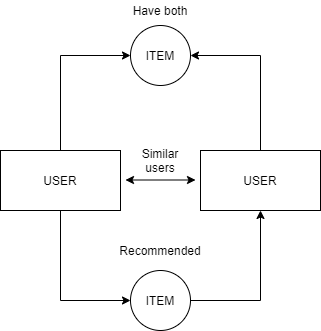
\includegraphics[width=0.4\textwidth]{CF.png}  
  \caption{ภาพรวมการกรองแบบร่วมกัน}
  \label{Fig:cf}
\end{figure}
การกรองแบบร่วม เป็นเทคนิคและนำโดยใช้ข้อมูลการโต้ตอบในอดีตที่ถูกบันทึกไว้ระหว่างยูสเซอร์และรายการเพื่อสร้างคำแนะนำใหม่ ๆ โดยข้อมูลเหล่านี้จะถูกเก็บไว้ในรูปแบบเมทริกซ์ที่เรียกว่า "user-item interactions matrix"
\newline
\begin{figure}[!h]
  \centering
  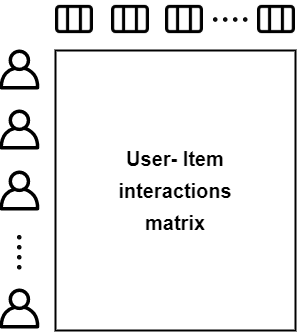
\includegraphics[width=0.3\textwidth]{colla_01.png}  
  \caption{เมทริกซ์การโต้ตอบยูสเซอร์ไอเทม}
  \label{Fig:colla_01}
\end{figure}

แนวคิดหลักที่เป็นกฎของการกรองแบบร่วมกันคือข้อมูลการโต้ตอบในอดีตในประมาณที่มากเพียงพอจะสามารถตรวจหาความคล้ายคลึงกันของยูสเซอร์กับไอเทมหรือยูสเซอร์กับยูสเซอร์ได้ 
คลาสของอัลกอริธึมการกรองแบบร่วมกันแบ่งออกเป็นสองประเภทย่อยที่โดยทั่วไปเรียกว่า อิงจากหน่วยความจำ (memory based) และ อิงจากโมเดล (model based) ในวิธีนี้การทำงานจะไม่มีการสันนิษฐานแบบจำลองแฝงแต่อัลกอริทึมจะทำงานโดยตรงกับข้อมูลการตอบโต้ยูสเซอร์และไอเทม ตัวอย่างเช่น ยูสเซอร์จะแสดงผลลัพธ์ของข้อมูลไอเทมเพื่อนบ้านที่ใกล้เคียงที่สุดเพื่อใช้ในการแนะนำ วิธีนี้จะมีความอคติต่ำในทางทฤษฎีแต่มีความแปรปรวนสูง 
และการอิงจากโมเดล วิธีนี้ถือว่าเป็นรูปแบบปฎิสัมพันธ์แฝง โมเดลนี้จะได้รับการฝึกให้สร้างค่าการตอบโต้ยูสเซอร์ไอเทมใหม่จากการแสดงยูสเซอร์และไอเทมของตัวเอง จากนั้นคำแนะนำใหม่สามารถทำได้โดยใช้โมเดลนี้ การทำนายจะมีความหมายทางคณิตศาสตร์ที่ยากต่อการตีความโดยมนุษย์ ดังนั้นวิธีการนี้ถือว่าเป็นวิธีที่มีความอคติสูงแต่มีความแปรปรวนต่ำ
\newline
\begin{figure}[!h]
  \centering
  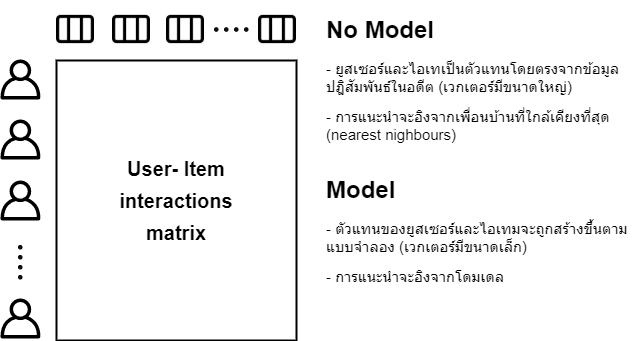
\includegraphics[width=0.8\textwidth]{colla_02.png}  
  \caption{ภาพรวมของกระบวนทัศน์วิธีการกรองร่วมกัน}
  \label{Fig:colla_02}
\end{figure}
\pagebreak

ข้อได้เปรียบหลักของการกรองแบบร่วมกันคือไม่ต้องการข้อมูลเกี่ยวกับยูสเซอร์หรือรายการเป็นตัวตั้งต้น ดังนั้นจึงสามารถใช้ได้ในหลายสถานการณ์ ยิ่งไปกว่านั้นยิ่งข้อมูลการโต้ตอบมีมากขึ้นเท่าใด คำแนะนำใหม่ก็จะยิ่งถูกต้องมากขึ้นเท่านั้น
แต่ถึงอย่างนั้นเนื่องจากไม่ต้องการข้อมูลในการตั้งต้นการพิจารณ์ข้อมูลเพื่อแนะนำจึงเกิดปัญหา นั่นคือ "cold start problem" ในทางปฎิบัติจึงเป็นไปไม่ได้ที่จะแนะนำสิ่งใดให้กับยูสเซอร์ใหม่หรือแนะนำรายการใหม่ให้กับยูสเซอร์ ยูสเซอร์และรายการที่มีข้อมูลการตอบโต้ที่น้อยเกินไปจะทำให้การแนะนำคลาดเคลื่อนเป็นอย่างมาก, ปัญหานี้สามารถแก้ไขได้หลายวิธีอย่างเช่น การแนะนำไอเทมแบบสุ่มให้กับยูสเซอร์ใหม่หรือแนะนำไอเทมใหม่กับยูสเซอร์แบบสุ่ม หรือการแนะนำไอเทมยอดนิยมให้กับยูสเซอร์ใหม่หรือไอเทมใหม่ให้กับยูสเซอร์ส่วนใหญ่ หรือการแนะนำชุดรายการให้กับยูสเซอร์ใหม่หรือรายการใหม่ไปยังกลุ่มยูสเซอร์ที่หลากหลายเป็นต้น

\pagebreak
\subsubsection{Memory Based}
\paragraph{User-user}
ในการแนะนำให้กับยูสเซอร์ วิธี user-user จะพยามระบุผู้ใช้ที่มีข้อมูลโปรไฟล์การโต้ตอบที่คล้ายคลึงกันมากที่สุด (เพื่อนบ้านที่ใกล้ที่สุด) เพื่อแนะนำรายการที่ได้รับความนิยมมากที่สุดให้บรรดาเพื่อนบ้านเหล่านี้ (หมายถึงยูสเซอร์ใหม่) วิธีนี้เรียกว่า "ผู้ใช้เป็นศูนย์กลาง" (user-centered)
สมมติว่าเราต้องการให้คำแนะนำสำหรับยูสเซอร์ใหม่ ขั้นแรกทุกคนจะถูกแทนที่ด้วยเวกเตอร์ของการโต้ตอบกับรายการ หลังจากนั้นเราสามารถคำนวนความคล้ายคลึงกันระหว่างยูสเซอร์ที่เราสนใจกับยูสเซอร์อื่น ๆ ทุกคน การวัดความคล้ายคลึงกันคือการที่ยูสเซอร์สองคนมีปฎิสัมพันธ์คลายคลึงกันในรายการเดียวกันนั่นหมายความว่าควรได้รับการพิจารณาว่าอยู่ใกล้กัน เมื่อคำนวนความคล้ายคลึงกับยูสเซอร์ทุกคนแล้ว เราสามารถเก็บ k nearest neighbour ไว้ให้กับยูสเซอร์ของเราจากนั้นแนะนำรายการที่ได้รับความนิยมมากที่สุดในบรรดารายการเหล่านี้
\newline
\begin{figure}[!h]
  \centering
  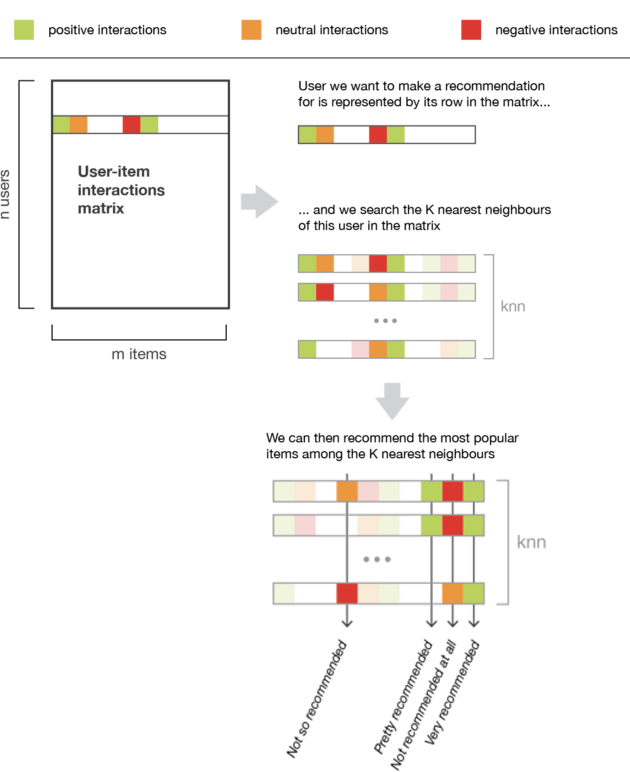
\includegraphics[width=0.8\textwidth]{content_user_user.png}  
  \caption{\cite[baptiste]{baptiste} วิธีการแบบ user-user}
  \label{Fig:content_user_user}
\end{figure}
\paragraph{Item-item}
การให้คะแนะนำใหม่แก่ยูสเซอร์แนวคิดของวิธี item-item คือการหารายการที่สอดคล้องกับรายการที่ยูสเซอร์มีรายการตอบโต้เป็นบวก (position) สองรายการซึ่งจะถือว่าคล้ายกันหากผู้ใช้ส่วนใหญ่ที่มีปฎิสัมพันธ์กับทั้งคู่ทำในลักษณะเดียวกัน วิธีนี้เรียกว่า "item-centered"
\newline
\begin{figure}[!h]
  \centering
  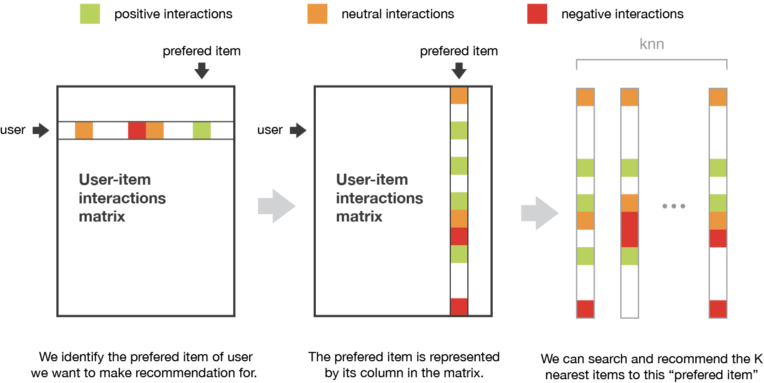
\includegraphics[width=1\textwidth]{content_item_item.png}  
  \caption{\cite[baptiste]{baptiste} วิธีการแบบ item-item}
  \label{Fig:content_item_item}
\end{figure}
\subsubsection{Model Based}
การกรองแบบร่วมกันโดยใช้โมเดล อาศัยข้อมูลการโต้ตอบยูสเซอร์ไอเทม และใช้โมเดลในการอธิบายข้อมูลการโต้ตอบเหล่านี้ ตัวอย่างเช่น อัลกอริธึมการแยกตัวประกอบเมทริกซ์ (matrix factorization) โดยสลายเมทริกซ์การโต้ตอบยูสเซอร์ไอเทมที่มีขนาดใหญ่และกระจายให้ให้เป็นตารางเมทริกซ์ที่มีขนาดเล็กและหนาแน่นจำนวนสองเมทริกซ์
\pagebreak
    

\subsection{การกรองแบบอิงเนื้อหา (Content Based Filtering)}
\begin{figure}[!h]
  \centering
  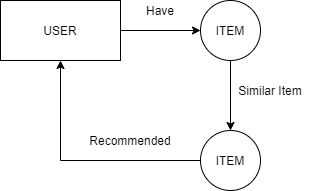
\includegraphics[width=0.4\textwidth]{CB.png}  
  \caption{ภาพรวมการกรองโดยอิงจากเนื้อหา}
  \label{Fig:CB}
\end{figure}
การกรองโดยอิงจากเนื้อหาต่างจากการกรองแแบบร่วมกันที่อาศัยข้อมูลการตอบโต้ยูสเซอร์และไอเทม การกรองโดยอิงจากเนื้อหาใช้ข้อมูลเพิ่มเติมเกี่ยวกับยูสเซอร์ และ/หรือ ไอเทม ยกตัวอย่างเช่นระบบแนะนำภาพยนต์ 
ข้อมูลเพิ่มเติมนี้อาจจะเป็น เพศ, อายุ, งาน หรือข้อมูลส่วนตัวอื่น ๆ ของยูสเซอร์ เพราะฉะนั้นแนวคิดนี้คือการพยามสร้างแบบจำลองตามคุณลักษณะเพื่อพยามอธิบายยูสเซอร์และไอเทม ตัวอย่างเช่น เมื่อพิจารณ์ภาพยนต์ เราจะพยามจำลองความจริงที่ว่าผู้หญิงมักจะให้คะแนนภาพยนต์บางเรื่องตามที่เพศหญิงชอบ และผู้ใช้จะให้คะแนนภาพยนต์บางเรื่องตามที่เพศตัวเองชอบ เป็นต้น หากทำการพิจารณ์จากตัวอย่างข้างต้นเราเพียงแค่ดูโปรไฟล์เพศเราก็สามารถแนะนำภาพยนต์ที่เพศนั้นๆ ชอบได้
\newline
\begin{figure}[!h]
  \centering
  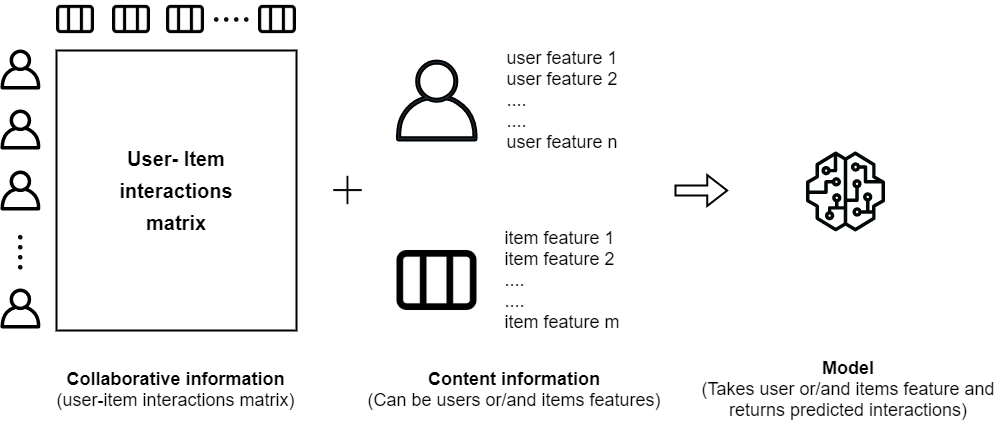
\includegraphics[width=1\textwidth]{content_01.png}  
  \caption{ภาพรวมของกระบวนทัศน์วิธีการกรองโดยอิงจากเนื้อหา}
  \label{Fig:content_01}
\end{figure}
วิธีการอิงจากเนื้อหานั้นไม่จะประสบปัญหา "cold start problem" น้อยกว่าวิธีการอิงแบบร่วมกัน ยูสเซอร์ใหม่หรือไอเทมใหม่สามารถอธิบายได้ตามลักษณะ (เนื้อหา) ของตัวมันเอง และคำแนะนำที่เกี่ยวข้องสามารถทำได้สำหรับเอนทิตีใหม่เหล่านี้ เฉพาะยูสเซอร์ใหม่หรือผู้ใช้ใหม่ที่มีคุณสมบัติที่ไม่เคยเจอมาก่อนเท่านั้นที่ได้รับผลกระทบจากข้อเสียนี้ แต่เมื่อมีข้อมูลมากเพียงพอปัญหานี้จะหมดไป
\pagebreak

\subsection{ระบบให้การแนะนำแบบผสม (Hybrid Recommendation)}
ระบบการแนะนำแบบผสม เป็นการประยุกต์ระบบแนะนำหลายหรือหลายข้อมูลเข้าด้วยกันเพื่อเพิ่มประสิทธิภาพในการทำนาย และแก้ไขปัญหาข้อด้อยของแต่ละเทคนิค


\section{Apache Airflow}
Apache airflow \cite{airflow} เป็นแพลตฟอร์มการจัดการเวิร์กโฟลว์แบบโอเพนซอร์สามารถเขียนโปรแกรมเพื่อกำหนดเวลาขั้นตอนการทำงานและตรวจสอบผ่านอินเทอร์เฟชผู้ใช้ได้
Airflow เขียนด้วยภาษา python และเวิร์กโฟลว์ถูกสร้างผ่านสคริปต์ python โดยได้รับการออกแบบภายใต้หลักการ "configuration as code" แม้ว่าแพลตฟอร์มอื่น ๆ ที่ใช้หลักการนี้จะอยู่ภายใต้มาร์กอัพ เช่น XML แต่การใช้ python ช่วยให้นักพัฒนานำเข้าไลบรารีและคลาสเพื่อช่วยในการสร้างเวิร์กโฟลว์ได้ง่ายและมีประสิทธิภาพมากยิ่งขึ้นกว่าการตั้งค่าโดด ๆ แบบ XML

Airflow ใช้กราฟ acyclic กำกับ (DAG) เพื่อจัดการระเบียบเวิร์ฟเฟลว์งาน และการอ้างอิงถูกกำหนดไว้ใน python จากนั้น airflow จะจัดการตั้งเวลาและดำเนินการ DAG ตามเวลาที่กำหนด (เช่น รายชั่วโมงรายวัน) หรือตามทริกเกอร์เหตุการภายนอก


\section{Docker}
Docker \cite{docker} เป็นเอ็นจิ้นที่มีการทำงานในลักษระจำลองสภาพวแดล้อมขึ้นมาบนเครื่องเซิรฟ์เวอร์เพื่อใช้ในการรันเซอร์วิสที่ต้องการ มีการทำงานคล้ายคลึงกับเครื่องเสมือน (virtual machine) เช่น MVWare, VirtualBox, XEN, KVM แต่ข้อแตกต่างที่ชัดเจนคือ เครื่องเสมือนที่กล่าวมาจำเป็นต้องจำลองทั้งระบบปฎิบัติการ (OS) เพื่อใช้งานและหากต้องการใช้บริการใด ๆ จำเป็นต้องติดตั้งเพิ่มบนระบบปฎิบัติการนั้น แต่สำหรับ docker แล้วจะใช้สิ่งที่เรียกว่าคอนเทนเนอร์ ในการจำลองสภาพแวดล้อมขึ้นมา เพื่อใช้งานสำหรับ 1 บริการ ที่ต้องการใช้งานเท่านั้น โดยไม่ต้องมีส่วนระบบปฎิบัติการเข้าไปเกี่ยวข้องด้วยเหมือนเครื่องเสมือนอื่น ๆ
\newline
\begin{figure}[!h]
  \centering
  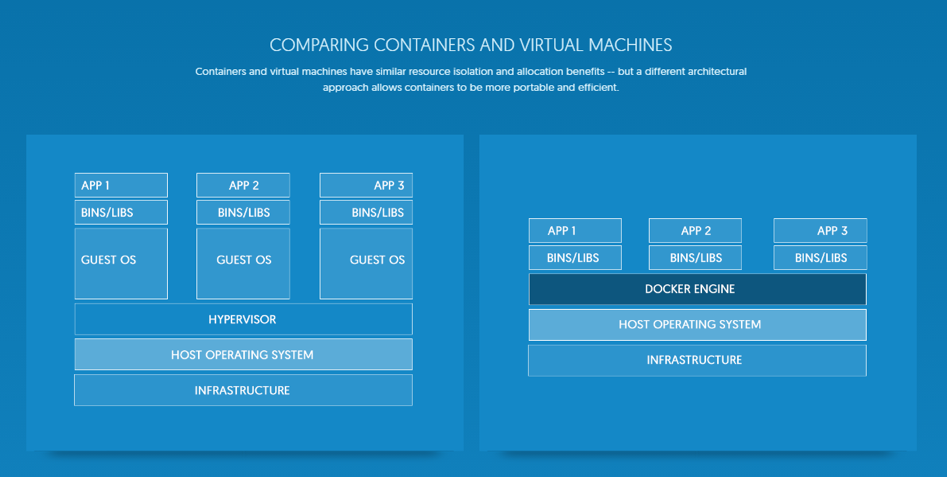
\includegraphics[width=1 \textwidth]{docker.png}  
  \caption{comparing container and virtual machines}
  \label{Fig:docker}
\end{figure}
โดย docker นั้นเป็นที่รู้จักกันอย่างแพร่หลายในช่วง 1-2 ปีที่ผ่านมานี้ เนื่องจากสามารถใช้งานได้อย่างสะดวกและตอบสนองความต้องการของผู้พัฒนาโปรแกรมหรือผู้ดูแลระบบ
\paragraph*{Docker image}
เป็นตัวต้นแบบของคอนเทนเนอร์ซึ่งภายในจะประกอบด้วยแอพพลิเคชั่นต่าง ๆ ที่มีการติดตั้งไว้เพื่อนใช้งานสำหรับบริการนั้น ๆ รวมทั้งมีการตั้งค่าต่าง ๆ ไว้อย่างเรียบร้อย จากนั้นจึงนำมาสร้างเป็นอิมเมจบนรีจิสทรีเพื่อนำมาใช้งานทั้งนี้ผู้ใช้งานสามารถสร้าง docker image ของตัวเองได้อีกด้วย
\paragraph*{Docker container}
เป็นกล่องเหสมือนซึ่งนำ docker image มาติดตั้งเพื่อให้สามารถใช้งานบริการที่ต้องการได้จากอิมเมจนั้น ๆ โดยในคอนเทนเนอร์แต่ละตัวจะมีการใช้งาน RAM, CPU ไฟล์ตั้งค่าต่าง ๆ เป็นของแต่ละคอนเทนเนอร์เอง


\section{การสกัดข้อมูล (Data Scraping)}
การสกัดข้อมูล \cite{choochart} เป็นเทคนิคในการเข้าถึงข้อมูลจากเว็บไซต์เพื่อที่หาและสกัดข้อมูลที่ต้องการ ในการสกัดข้อมูลจากข้อความที่ดึงมาจากเว็บไซต์สามารถใช้ไลบรารี่ beautifulsoup ของภาษา python เพื่อช่วยในการสกัดข้อมูลให้มีความง่ายขึ้นได้ กรณีที่เว็บไซต์ที่ทำงานโดยการเรนเดอร์หน้าเพจทั้งหน้าแล้วส่งมาให้ยูสเซอร์ (client) ราสามารถดึงข้อมูลของทั้งหน้ามาใช้ได้โดยตรงและสกัดข้อมูลจากที่กล่าวมาข้างต้น แต่บางเว็บไซต์ที่มีการทำงานแบบฝั่งไคลเอนต์ มีการแสดงผลข้อมูลเป็นแบบ Asynchronous ซึ่งทำให้ข้อมูลปรากฎขึ้นไม่พร้อมกัน โดยจะขึ้นอยู่กับการกระทำของยูสเซอร์เช่น คลิ๊กเปิด เลื่อนลงเพื่อโหลดฟีด จะไม่สามารถดึงข้อมูลทั้งหน้าได้จำเป็นต้องจำเป็นต้องแก้ปัญหาโดยทำการจำลองบราวเซอร์เพื่อจำลองการกระทำของยูสเซอร์ขึ้นมา
\subsection{Puppeteer}
Puppeteer เป็นไลบรารี่ Node ซึ่งมีอีพีไอระดับสูงเพื่อควบคุม Chrome หรือ Chromium ผ่านหน้าพัฒนา โดย puppeteer จะทำการรันเป็นเบราว์เซอร์ล่องหน (headless browser) หรือคือไม่มีอินเทอร์เฟซผู้ใช้งานแบบกราฟิกโดยเบราว์เซอร์ล่องหนสามารถควบคุมหน้าเว็บได้โดยอัติโนมัติในสภาพแวดล้อมที่คล้ายกับเว็บเบราว์เซอร์ แต่จำเดินการผ่านอินเทอร์เฟซบรรทัดคำสั่งหรือใช้การสื่อสารผ่านเครือข่าย มีประโยชน์เป็นอย่างมากสำหรับการทดสอบหน้าเว็บเนื่องจากสามารถแสดงผลและทำความเข้าใจ HTML ได้อีกทั้งยังสามารถประยุกต์ใช้เบราว์เซอร์ล่องหนในการสกัดข้อมูลจากเว็บไซต์ที่ต้องการผ่านการจำลองเสมือนเพื่อเข้าถึงข้อมูลที่ต้องการ 


\section{การประมวลผลภาษาธรรมชาติ (Natural Language Processing)}
การประมวลผลภาษาธรรมชาติ (NLP) \cite{diego} เป็นแขนงหนึ่งของสาขาปัญญาประดิษฐ์ (Artificial Intelligence) ที่ทำให้เครื่องจักรมีความสามารถในการอ่านทำความเข้าใจและเข้าใจความหมายของภาษามนุษย์ได้ กล่าวคือ NLP แสดงถึงการจัดการภาษามนุษย์โดยอัตโนมัติเช่นการพูด ข้อความ หรือแม้กระทั่งแนวคิดที่สนใจ โดยได้มีการนำไปประยุกต์ใช้ในแขนงมากมายเช่น ช่วยในการทำความเข้าใจและคาดการณ์กลุ่มของยูสเซอร์จากโปรไฟล์ของยูสเซอร์เหล่านั้น เป็นต้น

\subsection{Word Embedding}
Word Embedding \cite{lukkiddd} คือการจับบริบทของคำในเอกสารที่มีความคล้ายคลึงกับคำอื่น ๆ และแปลงคำให้เป็นตัวเลขในรูปแบบเว็กเตอร์ โดยถือเป็นหนึ่งในวิธีการสร้างฟีเจอร์จากคำวิธีหนึ่ง โดยทำการลดขนาดเว็กเตอร์ลงด้วย เช่น ทำการ word embedding กับคำว่า "I, liked, the, hotel" เราจะได้เวกเตอร์ออกมาคือ I[0.3, 0.2, 0.8, 0.1], liked[0.4, 1.2, 0.1, 0.9], the[1.3, -2.1, 0, 1.2], hotel[0.5, 1.4, 0.3, -0.4] เป็นต้น

\subsubsection{Word2Vec}
Word2Vec \cite{lukkiddd} Pre-trained weight model หรือแบบจำลองน้ำหนักที่ผ่านการเทรนมาล่วงหน้าแล้ว word2vec มีสองแบบที่สามารถใช้เพื่อทำ word embeddings คือ CBOW และ Skip-gram
\begin{enumerate}
  \item \textbf{Bag-of-Words Models (CBOW)} โดมเดลนี้จะทำนายคำถัดไปโดยอ้างอิงจาก n คำก่อนหน้าและ n คำต่อท้ายคำถัดไป ตัวอย่างเช่นประโยคต่อไปนี้ 
  
  \centerline{\emph{Lorem ipsum dolor sit amet}}
  
  CBOW จะทำนายคำ \emph{dolar} โดยให้อินพุต n = 2 ก่อนและหลังคำซึ่งจะได้ว่า \emph{Lorem, ipsum, sit} และ \emph{amet} คำเหล่านี้เรียกว่าบริบทของคำเป้าหมายและปริมาณจะเป็นพารามิเตอร์ของแบบจำลอง

  \item \textbf{Skip-gram} จากที่จะคาดเดาตามบริบทของคำ skip-gram จะทำนายบริบทแค่คำเดียว จากตัวอย่างก่อนหน้านี้เมื่อทำการทำนายด้วย skip-gram ตัว skip-gram จะพยามทำนายคำว่า \emph{Lorem, ipsum, sit} และ \emph{amet} โดยมีคำว่า \emph{dolar} เป็นอินพุต
\end{enumerate}

\subsection{Term Frequency-Inverse Document Frequency (TF-IDF)}
TFIDF \cite{cory} ใช้เพื่อชั่งน้ำหนักของคำสำคัญ (Keyword) ในเอกสารใด ๆ เพื่อกำหนดความสำคัญให้กับคำสำคัญเหล่านั้นตามจำนวนครั้งที่ปรากฎในเอกสาร หรือก็คือยิ่งคะแนน TF * IDF(น้ำหนัก) สูงเท่าไหร่คำนั้นก็จะสำคัญเท่านั้น ในทุกคำหรือคำศัพท์แต่ละคำจะมีคะแนน TF และ IDF อยู่เสมอ ผลคูณของคะแนน TF และ IDF ของคำหนึ่งจะเรียกว่าน้ำหนัก TF*IDF ของคำนั้น ๆ
\newline

ความถี่ (TF: Term Frequency) ของคำคือจำนวนครั้งที่ปรากฎในเอกสาร เมื่อทราบถึง TF แล้วเราจะสามารถบอกได้ว่ามีคำนั้นปรากฎในเอกสารบ่อยเท่าใด
\begin{equation}
  TF(t) = \text{จำนวนครั้งที่ } t \text{ ปรากฎบนเอกสาร } / \text{ จำนวนคำทั้งหมดในเอกสาร}
\end{equation}

ความถี่เอกสารผักผัน (IDF: Inverse Document Frequency) ของคำคือการวัดความสำคัญของคำเหล่านั้นในคลังข้อมูลคำ (Copus) ทั้งหมด
\begin{equation}
  IDF(t) = log_e (\text{จำนวนเอกสารทั้งหมด } / \text{ จำนวนเอกสารที่มีคำศัพท์อยู่ในนั้น})
\end{equation}

\begin{equation}
  W_{x, y} = TF_{x, y} \cdot log\left( \frac{N} {DF_{x}} \right)
\end{equation}
\begin{conditions}
  TF_{x, y}     &  frequency of x in y \\
  DF_{x}        &  number of documents containing x \\
  N             &  total number of document
\end{conditions}
เมื่อเราทำ TF-IDF แล้วเราสามารถเห็นความสำคัญของข้อความสำคัญได้


\section{การหาความสอดคล้องระหว่างสองสิ่ง}
ในการหาความสอดคล้องระหว่างสองสิ่ง \cite{selva} เราสามารถทำได้โดยใช้เทคนิคความคล้ายคลึงของโคไซน์ (Cosine Similarity ) 
\newline
\begin{equation}
  sim_{A, B} = \frac{A \cdot B} {||A||||B||} = \frac{\Sigma^{n}_{i=1} A_{i}B_{i}} {\sqrt{\Sigma^{n}_{i=1}A^{2}_{i}} \sqrt{\Sigma^{n}_{i=1}B^{2}_{i}}}
\end{equation}
\newline
ตัวอย่างข้อความ "backend developer", "senior software developer" เมื่อนำมาเปลี่ยนเป็นเมทริกซ์เทคนิคการนับคำ (count vectorizer) จะได้เมทริกซ์ [1, 1, 0, 0] และ [0, 1, 1, 1]
หลังจากมาหาความสอดคล้องจากการแทนค่าจากสมการดังกล่าวจะได้
\newline
\begin{equation}
  sim_{A, B} = \frac{(1\cdot0 + 1\cdot1 + 0\cdot1 + 0\cdot1)} {\sqrt{(1^{2} + 1^{2} + 0^{2} + 0^{2})} \sqrt{(0^{2} + 1^{2} + 1^{2} + 1^{2})}}
\end{equation}
\begin{equation}
  sim_{A, B} = \frac{1} {\sqrt{2} \sqrt{3}}
\end{equation}
ดังนั้นแล้วความสอดคล้องระหว่าง "backend developer" และ "senior software developer" คือ 0.408


\section{Support Vector Machine}
Support Vector Machine (SVG) \cite{cory2} เป็นเทคนิค Pattern Recognition แบบ Supervised Learning ถูกใช้ในเคส Classification และ Regression 
โดยภายในงานนี้ได้ถูกใช้เพื่อ Classification ตำแหน่งงานด้วยการสร้าง Hyper-plane ที่เหมาะสมที่สุด (Optimal)
เพื่อแยกข้อมูลสองกลุ่มด้วย Optimal Hyper-plane นั้น $w \times x - b = 0$ จะทำหน้าที่แบ่งข้อมูลสองกลุ่มออกจากกันด้วยมี Support Vector ทำหน้าที่เป็นกันชนระหว่างข้อมูลที่ใกล้กัน SVM จะสร้างพื้นที่การตัดสินใจขึ้นมา
หรือก็คือพื้นที่ระหว่าง $w \times x - b = 1$ และ $w \times x - b = -1$ โดยจะปรับให้ระยะห่างหรือความกว้างระหว่างทั้งสองนั้นมีค่าสูงที่สุด แต่บางกรณีข้อมูลไม่สามารถแบ่งแยกได้ด้วยเส้นตรง จำเป็นต้องแบ่งข้อมูลแบบ Non-linear ซึ่ง
SVM สามารถใช้ Kernel เข้ามาช่วยในการเปลี่ยนมิติของข้อมูลเพื่อให้สามารถแบ่งแยกข้อมูลทั้งสองกลุ่มได้ด้วย Linear Hyper-plan

\section{เว็บแอพพลิเคชั่น (Web Application)} 
Web Application \cite{margaret} ทำหน้าที่ในการเป็นช่องทางในการเชื่อมต่อระหว่างเว็บไซต์กับผู้ให้บริการไอพีไอจากที่อื่น เป็นตัวกลางที่ทำให้โปรแกรมสามารถประยุกต์เชื่อมต่อกับโปรแกรมประยุกต์อื่น ๆ ได้ เช่น google map ที่ทาง google ให้บริการให้ยูสเซอร์สามารถนำเว็บไซต์ของตนเองเชื่อมต่อกับแผนที่ของ google ได้

\subsection{จาวาสคริปต์ (Javascript)}
เป็นภาษาคอมพิวเตอร์ที่นิยมใช้ในการพัฒนาเว็บแอพพลิชั่น เนื่องจากจาวาสคริปต์มีความสามารถในการจัดการได้ทั้งฝั่งไคลเอนต์ (client) และฝั่งเซิร์ฟเวอร์ (server) ภาษาจาวาสคริปต์เป็นภาษาที่มีคุณสมบัติอะซิงโครนัส (asynchronous) ซึ่งแก้ไขปัญหาการขัดกันระหว่างคำสั่งที่ต้องรอในการรันคำสั่งถัดไปของภาษาที่เป็นซิงโครนัส (synchronous)

\subsection{วิว (Vue)}
Vue.js เป็นไลบรารี่จาวาสคริปต์ที่มุ่งเน้นไปที่เลเยอร์ของมุมมอง(view) สำหรับพัฒนามุมมองผู้ใช้(user interface) โดยในตัวไลบรารี่สามารถรองรับแอพพลิเคชั่นที่ซับซ้อนเช่นระบบ จัดการเส้นทาง(routing) ระบบจัดการสถาณะ(state) และการสร้าง(build)

\section{เอพีไอ (API)}
  Application Programming Interface (API) \cite{wiki api} คือส่วนต่อประสานโปรแรกมประยุกต์ เป็นวิธีการที่ระบบปฎิบัติการ, ไลบรารี และบริการอื่น ๆ เปิดให้โปรแกรมคอมเตอร์สามารถติดต่อเรียกใช้งานได้ โดยเอพีไอสร้างขึ้นจากส่วนสำคัญสองส่วนคือ
  \begin{enumerate}
    \item ข้อกำหนดที่จะอธิบายการแลกเปลี่ยนข้อมูลระหว่างโปรแกรม ที่ทำออกมาในลักษณะของเอกสาร เพื่อว่าคำร้องและการตอบสนองต้องเป็นอย่างไร
    \item ซอฟต์แวร์ที่เขียนขึ้นมาตามข้อกำหนดดังกล่าว และทำการเผยแพร่ออกไปให้ใช้งานได้
  \end{enumerate}
  
  โดยทั่วไปแล้วแอพพลิเคชั่นที่มีเอพีไอจะต้องถูกเขียนเป็นภาษาโปรแกรมมิ่ง และเพื่อการพัฒนาในอนาคต จึงจำเป็นต้องมีการตรวจสอบโครงสร้างของเอพีไอดังนั้น ผู้ออกแบบจึงต้องให้ความสำคัญกับการทดสอบ เพื่อตรวจสอบเงื่อนไขที่สามารถเกิดขึ้นได้จากการใช้งาน

  \subsection*{การใช้งานเอพีไอ} ปัจจุบันเอพีไอถูกใช้งานงานในแอพพลิเคชั่นเพื่อสื่อสารระหว่างไคลเอนต์และเซิร์ฟเวอร์ บริษัทยักใหญ่หลายบริษัทมีการเปิดให้บริการเอพีไอ เพื่อใช้งานภายนอก เช่น twitter, google, facebook โดยใครก็ตามที่สนใจนำบริการเหล่านี้ไปประยุกต์ใช้ สามารถส่งคำร้องเพื่อรับข้อมูลที่ต้องการ หรือถึงส่งคำร้องเพื่อขอบริการได้
    \paragraph*{ไลบรารีและเฟรมเวิร์ค} 
      โดยปกติแล้วเอพีไอ จะเกี่ยวข้องกับไลบรารีซอฟต์แวร์ เอพีไอจำเป็นต้องอธิและข้อกำหนด เอพีไอเดียวสามารถมีการใช้งานได้หลากหลาย (หรือไม่มีเลย) ในรูปแบบของไลบรารี่ต่าง ๆ ที่ใช้อินเทอร์เฟชการเขียนโปรแรกมร่วมกัน การแยกเอพีไอออกจากการนำไปใช้งาน สามารถทำให้โปรแกรมที่เขียนภาษาหนึ่งใช้ไลบรารีที่เขียนด้วยอีกภาษาหนึ่งได้ ตัวอย่างเช่นเนื่องจากภาษา scala และภาษา java คอมไล์เป็น bytecode ที่เข้ากันได้ นักพัฒนา scala จึงสามารถใช้ประโยชน์จากภาษาโปรแกรมที่เกี่ยวข้องกับเอพีไอภาษา Java ได้เป็นต้น \par
    \paragraph*{ระบบปฎิบัติการ}
      เอพีไอสามารถระบุอินเทอร์เฟซระหว่างแอพพลิเคชั่นและระบบปฎิบัติการได้ ตัวอย่างเช่น microsoft ได้สร้างความมุ่งมั่นอย่างยิ่งต่อเอพีไอที่เข้ากันได้กับไลบรารี่ windows api (win32) ดังนั้นแอพพลิเคชั่นรุ่นเก่าอาจทำงานบน windows เวอร์ชั่นใหม่โดยใช้งานตั้งค่าเฉพาะปฎิติบัติการที่เรียกว่า "โหมดความเข้ากัน" เป็นต้น
    \paragraph*{รีโมทเอพีไอ}
      รีโมทเอพีไอถูกใช้ให้นักพัฒนาสามารถเข้าควบคุมทรัพยากรผ่านทางโปรโตคอลเพื่อให้มีมาตราฐานการสือสารเดียวกัน ถึงแม้ว่าจะเป็นคนละเทคโนโลยี เช่น ฐานข้อมูลเอพีไอสามารถอนุญาตให้นักพัฒนาเข้ามาดึงข้อมูลในฐานข้อมูลได้หลากหลายชนิดได้ผ่านฟังค์ชั่นเดียวกัน เพราะฉะนั้นรีโมทเอพีไอจึงถูกใช้บ่อยในงานรักษาด้วยทำทำงานที่ฝั่งไคลเอนต์ให้ไปดึงข้อมูลจากเซิร์ฟเวอร์กลับลงมาทำงาน
    \paragraph*{เว็บเอพีไอ}
      เว็บเอพีถูกใช้กันอย่างแพร่หลายในปัจจุบัน เนื่องจากเป็นเอพีไอที่อยู่ในกลุ่มของ HTTP และขยายออกไปสู่รูปแบบต่าง ๆ เช่น XML และ JSON ซึ่งโดยรวมแล้วจะอยู่บนเว็บเซอร์วิซ เช่น SOUP หรือ REST เป็นต้น

  \subsection*{ตัวอย่างเอพีไอที่นิยมในปัจจุบัน}
    \begin{enumerate}
      \itemsep0em 
      \item \textbf{Google Maps API} เปิดให้ใช้งานเพื่อนำเอาแผนที่ของ Google มาลงใน webpage โดยอาศัย JavaScript หรือ Flash
      \item \textbf{Youtube API} Google ยอมให้ developer สามารถนำเอา Clip video บน YouTube ไปลงใน website หรือ application ได้
      \item \textbf{Flickr API} เพื่อให้ developer สามารถเข้าถึง คลังรูปภาพใน community
      \item \textbf{Twitter API} มี REST API ให้ค้นหา แล้วตรวจสอบข้อมูล trends ได้
      \item \textbf{Amazon product advertising API} เปิด API ให้ใช้ค้นหาสินค้า และ การโฆษณาผ่านทาง website
    \end{enumerate}

  \subsection{Flask}
  เฟลค คือเว็บเฟรมเวิร์คเป็นเฟรมเวิร์คที่เขียนขึ้นมาสำหรับใช้งานในภาษา Python   ไพทอน (ไพธอน)  เพื่อใช้ในการสร้างเว็บไซต์ ทำให้ภาษาไพธอนนั้น มีความสามารถในการจัดการกับเว็บไซต์ซึ่งทำให้มึความสามารถคล้ายๆภาษา PHP (พีเอชพี)  ซึ่งแทบจะใช้แทนกันได้เลย  ในปัจจจุบันมีผู้ใช้ Flask Framework ค่อนข้างจะเยอะมากซึ่งเป็นผลมาจากการใช้งานที่ง่ายและผนวกกับมีผู้ใช้ภาษาไพธอนเพิ่มขึ้นนั่นเอง
    \paragraph*{Python} ภาษาโปรแกรม Python \cite{python} คือภาษาโปรแกรมคอมพิวเตอร์ระดับสูง โดยถูกออกแบบมาให้เป็นภาษาสคริปต์ที่อ่านง่าย  โดยตัดความซับซ้อนของโครงสร้างและไวยกรณ์ของภาษาออกไป ในส่วนของการแปลงชุดคำสั่งที่เราเขียนให้เป็นภาษาเครื่อง Python มีการทำงานแบบ Interpreter คือเป็นการแปลชุดคำสั่งทีละบรรทัด เพื่อป้อนเข้าสู่หน่วยประมวลผลให้คอมพิวเตอร์ทำงานตามที่เราต้องการ นอกจากนั้นภาษาโปรแกรม Python ยังสามารถนำไปใช้ในการเขียนโปรแกรมได้หลากหลายประเภท โดยไม่ได้จำกัดอยู่ที่งานเฉพาะทางใดทางหนึ่ง (General-purpose language) จึงทำให้มีการนำไปใช้กันแพร่หลายในหลายองค์กรใหญ่ระดับโลก เช่น Google, YouTube, Instagram, Dropbox และ NASA เป็นต้น 

% \section{กระบวนการวัด (Measurement Process)}
% การวัดผลซอฟต์แวร์มีบทบาทสำคัญในกิจกรรมการพัฒนาซอฟต์แวร์ทั้งหมด พอลกู๊ดแมนผู้เขียนแนวทางปฏิบัติของเมตริกซอฟต์แวร์อ้างว่าบทบาทของเมตริกซอฟต์แวร์คือการช่วยให้วิศวกรและผู้จัดการสามารถอยู่รอดได้ในสภาพแวดล้อมทางธุรกิจในปัจจุบัน \cite[paul goodman]{paul} การวัดที่ได้มาจากการวัดผลคือตัวเลขที่ใช้ในการสร้างเมตริกและเมตริกคือตัวเลขที่เปลี่ยนเป็นข้อมูล ผู้จัดการจำเป็นต้องมีพื้นฐานในการประเมินคุณภาพผลิตภัณฑ์และวิเคราะห์ประเด็นหรือปัญหาและเป็นพื้นฐานสำหรับการควบคุมเชิงปริมาณของกระบวนการจัดการโครงการและวิศวกรรม นอกจากนี้การวัดผลยังให้ข้อมูลเชิงลึกที่ผู้จัดการต้องใช้ในการตัดสินใจที่สำคัญต่อความสำเร็จของโครงการ \cite[PSM Group]{psm group} โปรแกรมการวัดผลที่มีประสิทธิภาพช่วยและทำให้พวกเขาประสบความสำเร็จโดยการพัฒนาแผนการที่ทำได้
% \subsection{Planning}
\chapter{วิธีการทดลอง}
\label{chapter:experiment}


% Set Function Names
\SetKwFunction{FMain}{Main}
\SetKwFunction{FLogin}{Login}
\SetKwFunction{FUrl}{GetUrl}
\SetKwFunction{FData}{getData}

ในบทนี้จะกล่าวถึงขั้นตอนและกรอบการทำงานในการพัฒนาระบบแนะนำตำแหน่งงาน การจัดการข้อมูล และการพัฒนาเว็บแอพพลิเคชั่น โดยมีจุดประสงค์เพื่อทำให้ระบบแนะนำตำแหน่งงานสามารถทำงานได้อย่างมีประสิทธิภาพสามารถใช้งานได้จริง รวมถึงอภิปรายภาพรวมระบบทั้งหมด



\section{สถาปัตยกรรมสำหรับไปป์ไลน์ข้อมูล}
สถาปัตยกรรมที่ผู้เขียนเลือกใช้นั้นเป็นเทคโนโลยีโอเพนซอร์สทั้งหมดเพื่อทำให้ทุกขั้นตอนของท่อส่งข้อมูลสามารถทำงานจริงได้ในระยะยาวโดยคำนึงถึงต้นทุนและประสิทธิภาพที่ตามมา
\subsection{โครงสร้างพื้นฐานของระบบ} 
บนเครื่องเซิร์ฟเวอร์นั้นทางผู้เขียนได้เลือกเทคโนโลยี docker เข้ามาใช้ในการจำลองเครื่องเสมือนโดยแบ่งบริการเป็นคอนเทนเนอร์ต่าง ๆ 
เพื่อความง่ายในการควบคุมและจัดการตัวบริการนั้น ๆ อีกทั้งสามารถสเกลได้เมื่อบริการนั้นมีการใช้งานในปริมาณที่มากในอนาคตและง่ายต่อการติดตั้งเมื่อมีการย้ายเซิร์ฟเวอร์
โดยบริการที่ทำงานอยู่บน docker เช่น ฐานข้อมูล ระบบจัดการตารางาน ระบบสกัดข้อมูล โมดูลทำความสะอาดและแปลงข้อมูล โมดูลจำแนกประเภทกลุ่มของข้อมูล ระบบแนะนำ บริการเว็บเซอร์วิส เป็นต้น
\newline

\begin{figure}[!h]
  \centering
  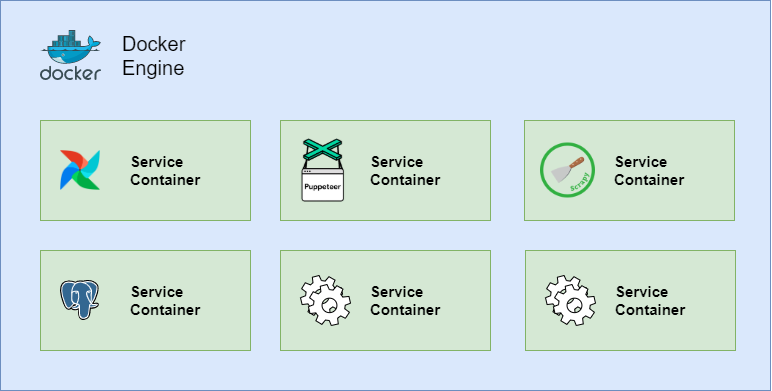
\includegraphics[width=0.8\textwidth]{structure_docker.png}  
  \caption{รูปภาพกรอบการทำงาน บริการที่ทำงานอยู่บน docker engine}
  \label{Fig:data-collection}
\end{figure}

\subsection{แพลตฟอร์มจัดการเวิร์กโฟลว์}
Apache airflow เป็นแพลตฟอร์มการจัดการเวิร์กโฟลว์สามารถกำหนดเวลาหรือขั้นตอนการทำงานได้ด้วยการเขียนโปรแกรมผ่าน python โดยแพลตฟอร์มนี้ถูกต้องตั้งเป็นบริการอยู่บน docker engine 
เพื่อทำการควบคุมตารางการทำงานและโฟลว์ของเคนเทนเนอร์อื่น ๆ โดยมีลำดับการทำงานดังนี้


\subsection{การรวบรวมข้อมูล}
การรวบรวมข้อมูลมีการรวบรวมจากสองแหล่งคือเว็บไซต์ linkedin และเว็บไซต์ indeed โดยทั้งสองเว็บไซต์นี้มีขั้นตอนการสกัดและรวบรวมไม่เหมือนกันโดยเว็บไซต์ linkedin มีความซับซ้อนและความยากในการสกัดข้อมูลมากเนื่องจากเป็นเว็บไซต์ระดับโลกที่มีการป้องกันบอทและการเข้าถึงต่าง ๆ ที่ไม่ใช่มนุษย์อีกทั้งหน้าเว็บยังมีการทำงานเป็นแบบ client-side rendering ซึ่งจำเป็นต้องใช้การจำลองเสมือนมนุษย์มาทำหน้าที่เป็นบอทผ่านไลบรารี่ puppeteer ส่วนเว็บไซต์ indeed เนื่องจากมีการทำงานเป็น server-side rendering จึงสามารถดึงข้อมูลได้ตรงจากการสร้างคำร้องไปที่เซิฟเวอร์และเซิฟเวอร์จะตอบกลับมาเป็นหน้าเว็บเพจที่เป็น static
\newline
\begin{figure}[!h]
  \centering
  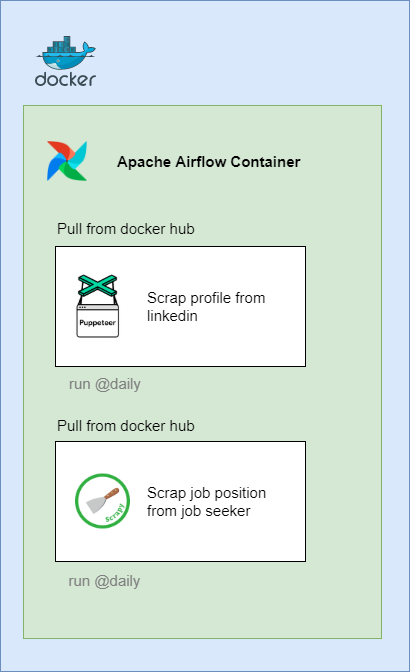
\includegraphics[height=0.7\textwidth]{structure_airflow.png}  
  \caption{รูปภาพกรอบการทำงาน การรวบรวมข้อมูลภายใต้ Airflow}
  \label{Fig:data-collection}
\end{figure}
ทั้งนี้การสกัดข้อมูลจำเป็นต้องมีคำสำคัญหรือเป้าหมายที่เจาะจงในการสกัดข้อมูล ทางผู้จัดทำได้รวบรวมตำแหน่งงานทางเทคโนโลยีสารสนเทศโดยอิงจาก CompTIA certification roadmap โดยแบ่งสายงานทางเทคโนโลยีสารสนเทศเป็นทั้งหมด 8 สายงานและ 62 ตำแหน่งดังนี้
\newpage

\begin{enumerate}
  \item \textbf{service and infrastructure}
  \newline
  helpdesk,
  system admin, 
  virtualization engineer, 
  system engineer, 
  system architect
    
  \item \textbf{network technology}
  \newline
  network technician, 
  network analyst, 
  telecommunication, 
  network security, 
  network admin, 
  network engineer

  \item \textbf{it business and strategy}
  \newline
  it operation, 
  business architect, 
  business analyst, 
  policy advisor, 
  policy consultant, 
  enterprise architect

  \item \textbf{it management}
  \newline
  it manager, 
  it deputy director, 
  it director, 
  project manager, 
  program manager, 
  cto, 
  cio

  \item \textbf{information security}
  \newline
  security trainee, 
  security technician, 
  security analyst, 
  security manager, 
  security engineer, 
  security architect, 
  it auditor, 
  risk compliance, 
  incident, 
  forensics, 
  malware developer

  \item \textbf{devops and cloud technology}
  \newline
  sysops engineer, 
  devops admin, 
  devops engineer, 
  reliability engineer, 
  devops consultant, 
  cloud engineer, 
  cloud architect

  \item \textbf{storange and data}
  \newline
  data center, 
  data analyst, 
  database admin, 
  business intelligence, 
  data warehouse, 
  data scientist, 
  database architect, 
  data engineer, 
  database engineer

  \item \textbf{software development}
  \newline
  software developer, 
  software tester, 
  software support, 
  applications developer, 
  qa, 
  web developer, 
  applications security, 
  web manager, 
  software engineer, 
  software architect, 
  software system architect
\end{enumerate}

\begin{figure}[!h]
  \centering
  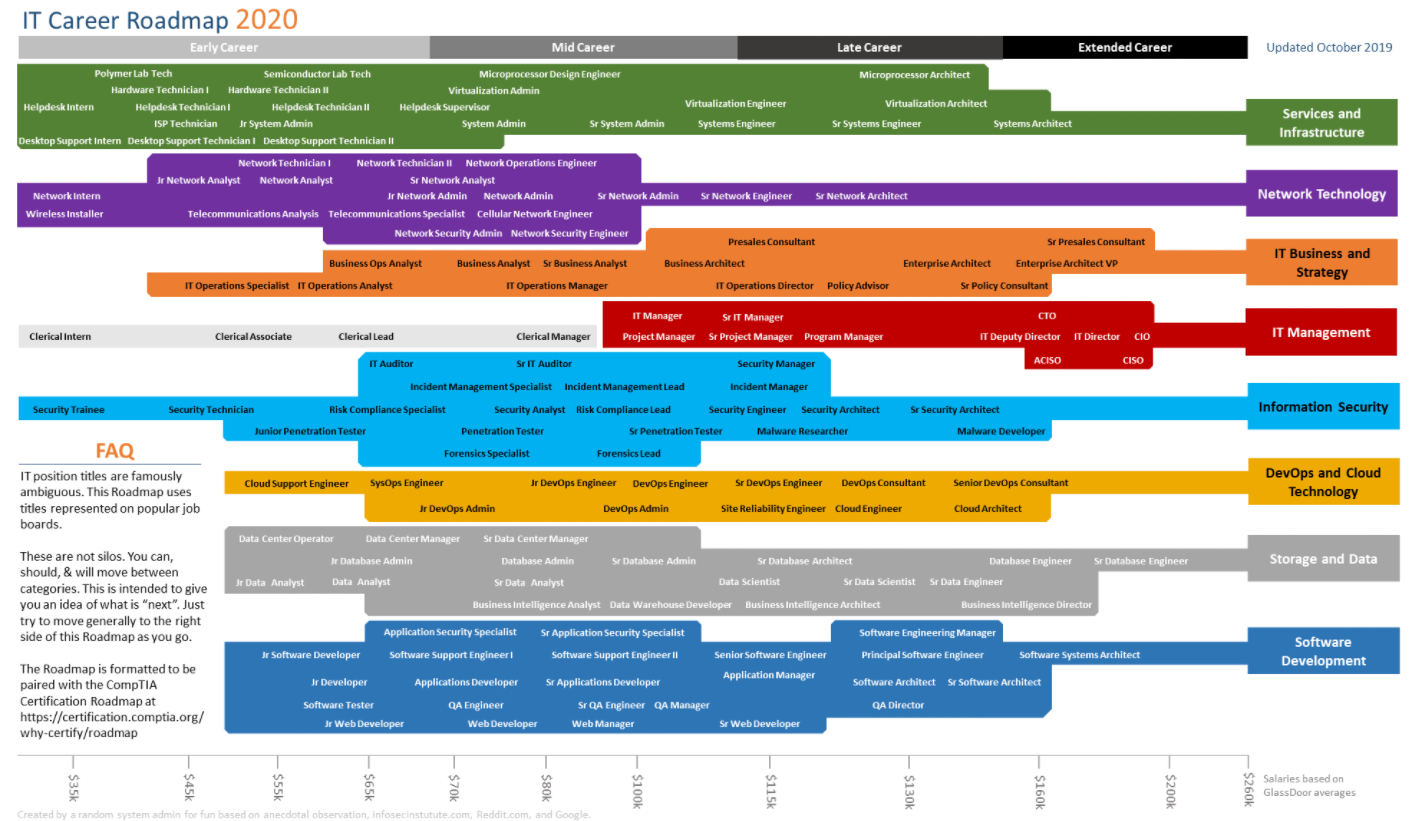
\includegraphics[width=1\textwidth]{chapter3/it_roadmap.png}  
  \caption{it roadmap}
  \label{Fig:it-roadmap}
\end{figure}
\newpage

\subsubsection{Linkedin}
การสกัดข้อมูลโปรไฟล์ผู้ใช้งานลิงค์อินจะใช้ไลบรารี่ puppeteer มาใช้ในการจำลองการกระทำของมนุษย์โดยมีกระบวนการหลักทั้งหมดสามขั้นตอนคือ
\begin{enumerate}
  \item การกำหนดรายการคำสั่งสำหรับการสกัดข้อมูล
  \begin{figure}[!h]
    \centering
    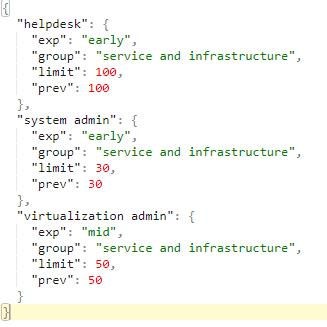
\includegraphics[width=0.4\textwidth]{chapter3/order.jpg}  
    \caption{ไฟล์รายการคำสั่งสกัดข้อมูลบางส่วน}
    \label{Fig:scrap-order}
  \end{figure}
  \item สกัดยูอาร์แอลโปรไฟล์ผู้ใช้จากการค้นหาผ่านคำสำคัญที่กำหนดในรายการคำสั่ง
  \item สกัดข้อมูลโปรไฟล์ผู้ใช้จากการเข้าสู่หน้าหลักโปรไฟล์ผ่านยูอาร์แอลที่สกัดมาจากขั้นตอนก่อนหน้า
\end{enumerate}

\begin{algorithm}
\DontPrintSemicolon
  \SetKwProg{Fn}{Function}{:}{}
  \Fn{\FMain{$order$}}{
    Login(env.username, env.password)\;
    GetUrl()\;
    GetData()\;
  }

  \SetKwProg{Fn}{Function}{:}{}
  \Fn{\FLogin{$username$, $password$}}{
    \eIf{exist cookies}{
      login with cookie\;
    }{
      login with username, password form\;
    }
    save cookie\;
  }

  \SetKwProg{Fn}{Function}{:}{}
  \Fn{\FUrl{}}{
    read order\;
    read backlist\;
    \If{not exist backlist}{
      generate backlist file from order\;
    }
    \While{order}{
      profiles = []\;
      \While{order.keyword}{
        search keyword\;
        scroll all page\;

        urls = querySelectorAll(all profile).href\;
        urls = backlist filter(urls)\;
        urls = realurl filter(urls)\;

        profiles.push(url)\;
      }
      save profiles to file\;
      update order file\;
      update backlist file\;
    }
  }

  \SetKwProg{Fn}{Function}{:}{}
  \Fn{\FData{}}{
    read url files
    \While{files}{
      data = []\;
      \While{files.url}{
        goto url\;
        validate page is exist\;
        scroll all page\;
        scrap name\;
        scrap about\;
        scrap experience\;
        scrap skill\;
        scrap interest\;

        data.push({name, about, experience, skill, interest})\;
      }
      save data to file\;
    }
  }

  \caption{Scrap profile algorithms}
\end{algorithm}

\subsubsection{Indeed}
การสกัดข้อมูลตำแหน่งงานจากเว็บไซต์อินดีดจะใช้เฟรมเวิร์ค scrapy มาใช้ในการรวบรวมข้อมูลจากรีเครสที่ส่งไปเพื่อค้นหาตำแหน่งงานจากคำสำคัญที่กำหนดไว้ โดยจะมีขั้นตอนการทำงานหลักสามขั้นตอนคือ
\begin{enumerate}
  \item การกำหนดรายการคำสั่งสำหรับการสกัดข้อมูล
  \begin{figure}[!h]
    \centering
    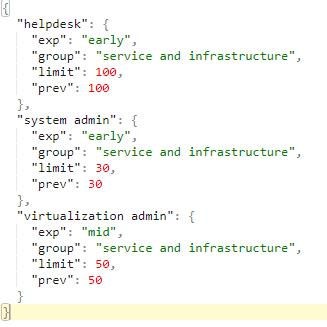
\includegraphics[width=0.4\textwidth]{chapter3/order.jpg}  
    \caption{ไฟล์รายการคำสั่งสกัดข้อมูลบางส่วน}
    \label{Fig:scrap-order}
  \end{figure}
  \item สกัดยูอาร์แอลตำแหน่งงานจากการค้นหาผ่านคำสำคัญที่กำหนดในรายการคำสั่ง
  \item สกัดข้อมูลหน้าตำแหน่งงานจากการเข้าสู่หน้าตำแหน่งงานจากยูอาร์แอลที่สกัดมาจากขั้นตอนก่อนหน้า
\end{enumerate}


\subsection{การจัดการข้อมูล}
หลังจากทำการรวบรวมข้อมูลจากทั้งสองแหล่ง (linkedin, indeeed) และบันทึกเป็นรูปแบบไฟล์อยู่ในทะเลสาบข้อมูลแล้ว airflow จะทำการรันและเริ่มกระบวนการทำความสะอาดข้อมูล(Data cleansing) โดยเป็นกระบวนการตรวจสอบแก้ไขหรือลบรายการข้อมูลที่ไม่ถูกต้องหรือไม่สอดคล้องออกจากชุดข้อมูลโดยมีขั้นตอนดังนี้
\begin{enumerate}
  \item ตรวจสอบฟอร์แมทและความถูกต้องของไฟล์ข้อมูล
  \item ลดรูปข้อมูลที่ซ้ำกัน ถ้าข้อมูลระบุกลุ่มที่แตกต่างกันให้รวมกลุ่มนั้นเป็นหลายรายการในข้อมูลเดียว
  \item ลบข้อมูลที่ไม่มีฟีเจอร์สำคัญคือฟีเจอร์ about และ skill
  \item ข้อมูลที่ผ่านขั้นตอนทั้งหมดจะถูกบันทึกลงฐานข้อมูลโดยมีรูปแบบที่ชัดเจนและพร้อมใช้งาน
\end{enumerate}

\begin{figure}[!h]
  \centering
  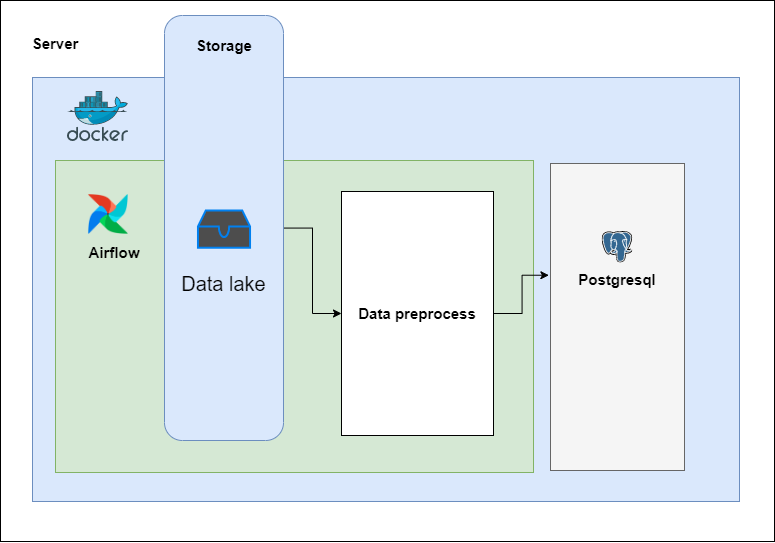
\includegraphics[width=0.8\textwidth]{structure_preprocess.png}  
  \caption{รูปภาพโฟลว์การทำงานของการจัดการข้อมูล}
  \label{Fig:data-collection}
\end{figure}



\subsection{การเทรนโมเดลแบ่งกลุ่มสายงาน}
  ในการเทรนโมเดลมีขั้นตอนหลายอย่างที่ต้องคำนึงถึง เพื่อให้โมเดลมีความแม่นยำในการแบ่งสายงาน จึงจำเป็นต้องนำเทคนิคต่าง ๆ มาประยุกต์ใช้ทั้งกับในด้านข้อมูลและด้านโมเดล โดยเทคนิคหลักที่นำมาใช้มีดังนี้
  \subsubsection*{การทำความสะอาดข้อมูล}
    ก่อนขั้นตอนการเทรนโมเดล ข้อมูลจำเป็นต้องอยู่ในรูปแบบที่เหมาะสมต่อการใช้ในการเทรนโมเดลมากที่สุดโดยขั้นตอนการ "clean data" จะประกอบไปด้วยขั้นตอนง่ายๆ ทั่วไปอย่างเช่น 
    \begin{enumerate}
      \item การเปลี่ยนข้อมูลให้เป็นตัวเล็ก อักขระพิเศษทั้งหมด ลบตัวอักษรโดด ลบแท็ก ลบช่องว่างที่เกินกำหนด
      \item การใช้ "stopword" คัดกรองคำที่ไม่จำเป็นออกจากข้อมูล
      \item ใช้เทคนิค"Lemmatizer" หรือการลดรูปคำให้เป็นคำรากศัพท์เช่น "am", "are", "is" จะถูกเปลี่ยนเป็น "be" 
      \item ใช้เทคนิค "Tokenize" หรือเทคนิคการแบ่งคำมาแบ่งข้อมูลให้อยู่ในรูปแบบโทเค็นหรือในรูปแบบคำต่อคำ
      \item พิจารณ์รูปแบบของคำที่สะกดผิดเช่น "cool", "kewl", "cooool"
    \end{enumerate}
    
  \subsubsection*{การสร้างโครงสร้างของคำ}
  เมื่อทำความสะอาดข้อมูลแล้วจะสังเกตุว่าข้อมูลยังมีการกระจายที่ยังไม่แน่นอนและไม่สามารถแยกแยะด้วยตาเปล่าได้ เทคนิคต่อไปนี้เป็นการทำให้ข้อมูลมีความชัดเจนมากยิ่งขึ้นโดยมีขั้นตอนดังนี้
  \begin{figure}[!h]
    \centering
    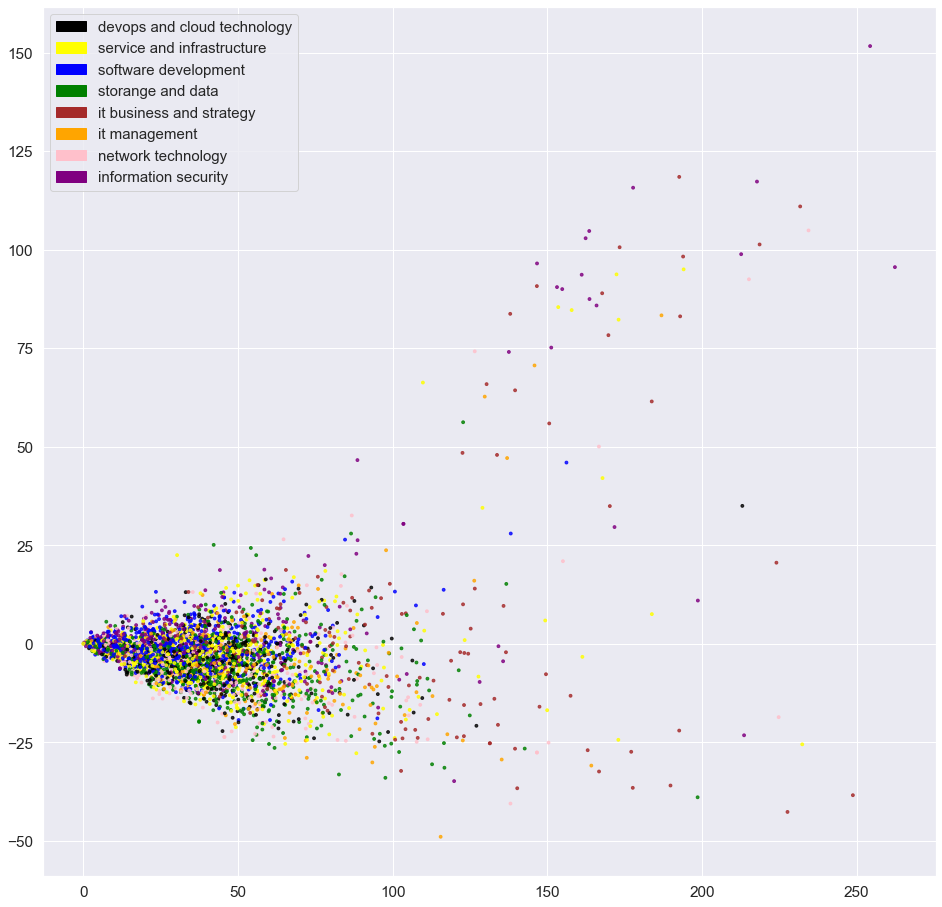
\includegraphics[width=1\textwidth]{chapter3/pca_counts.png}  
    \caption{PCA vector ของตำแหน่งงานเมื่อทำความสะอาดข้อมูลแล้ว}
    \label{Fig:pca-count}
  \end{figure}

  \paragraph*{TF-IDF} เพื่อช่วยให้โมเดลสามารถโฟกัสความหมายของคำได้จึงได้นำเทคนิค "TF-IDF (Term Frequency, Inverse Document Frequency)" เข้ามาใช้ในการให้น้ำหนักคำตามความหายากในชุดข้อมูล และลดคำที่เกิดขึ้นบ่อยเกินไปแล้วไปเพิ่ม noise ให้กับข้อมูลโดยรวม \par
  \begin{figure}[!h]
    \centering
    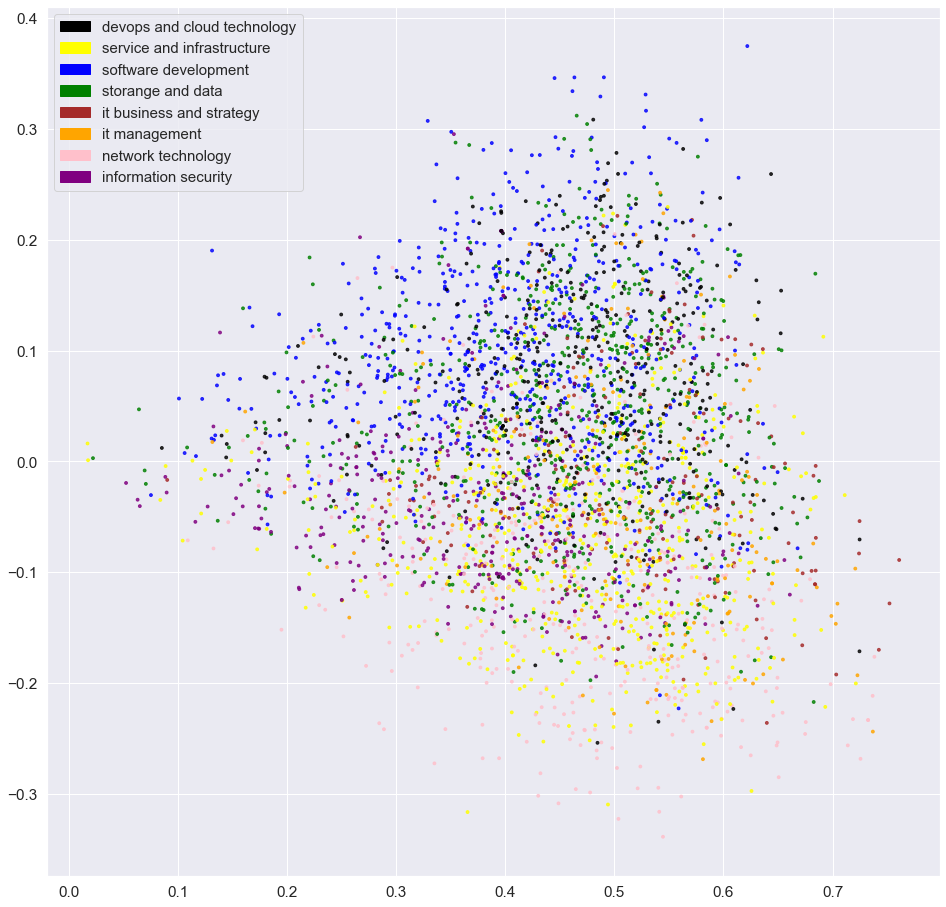
\includegraphics[width=1\textwidth]{chapter3/pca_tfidf.png}  
    \caption{PCA vector ของตำแหน่งงานเมื่อทำการให้น้ำหนักแก่คำแล้ว}
    \label{Fig:pca-tfidf}
  \end{figure}

  \paragraph*{Word2Vec} ถึงจะสามารถจัดการกับความถี่ของคำได้แล้ว แต่อย่างไรก็ตามมีความเป็นไปได้มากว่า หากเราปรับใช้โมเดลนี้เราจะพบคำศัพท์ที่เราไม่เคยเห็นในชุดข้อมูลของเรามาก่อน รุ่นก่อนหน้านี้อาจไม่สามารถจำแนกคำเหล่านี้ได้อย่างถูกต้องแม้ว่าคำจะเป็นคำที่คล้ายกันมากในการเทรนก็ตาม เพื่อแก้ปัญหานี้ การจับความหมายของคำ "semantic meaning of word" โดยเครื่องมือที่ใช้เพื่อจับความหมายเรียกว่า "Word2Vec" \par
    \subparagraph{pre-trained words} word2vec เป็นเทคนิคในการการฝังคำอย่างต่อเนื่อง(continuous embeddings) โดยเรียนรู้จักการอ่านข้อความจำนวนมากและจดจำคำที่มีแนวโน้มที่ปากฎในบริบทที่คล้ายคลึงกัน หลังจากที่เทรนมามากพอแล้วจะสร้างเวกเตอร์ 300 มิติ สำหรับแต่คำแต่ละคำในคำศัพท์ โดยคำที่มีความหมายใกล้เคียงกันจะมีระยะใกล้เคียงกัน
    โดยผู้จัดทำได้นำ pre-trained ของ "GoogleNews" ที่ประกอบไปด้วยเวกเตอร์ของคำมากกว่า 3 ล้าน หลังจากการทำ word embeddings ด้วย word2vec แล้วจะสังเกตุว่าการกระจายตัวมีความแน่นหนาขึ้นแต่การแบ่งแยกสายงานไม่แตกต่างจากการทำ TFIDF มากนัก
    \begin{figure}[!h]
      \centering
      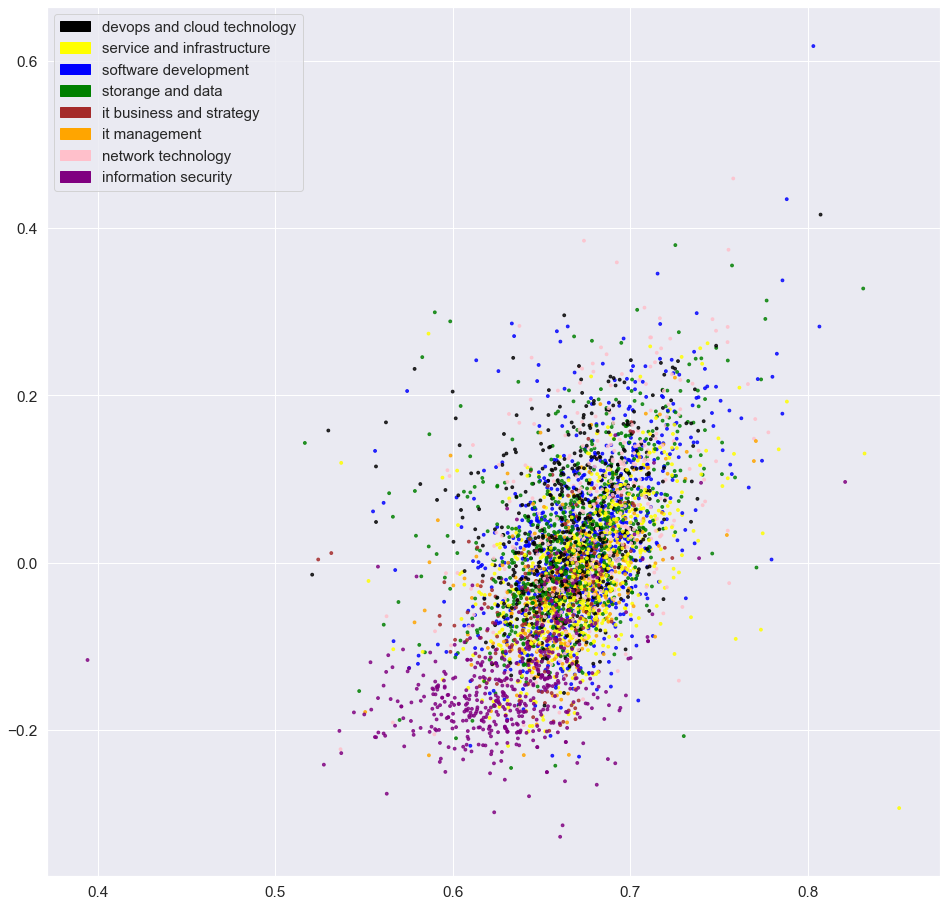
\includegraphics[width=0.8\textwidth]{chapter3/pca_word2vec.png}  
      \caption{PCA vector ของตำแหน่งงานผ่านเทคนิค word2vec}
      \label{Fig:pca-tfidf}
    \end{figure}
  
  \newpage
  หลังจากที่ข้อมูลอยู่ในรูปแบบที่พร้อมใช้งานแล้วจึงนำข้อมูลมาทำการสร้างโมเดลแบ่งกลุ่มตำแหน่งงาน โดยกลุ่มจะถูกแบ่งออกเป็นทั้งหมด 8 กลุ่มใหญ่และ 62 ตำแหน่งงาน \cite[CompTIA]{comptia} โดยมีลักษณะดังนี้\newline

  \begin{figure}[!h]
    \centering
    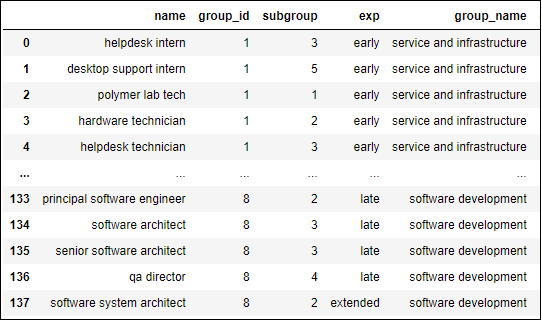
\includegraphics[width=0.7\textwidth]{structure_comptia.png}  
    \caption{กลุ่มงานทางไอที}
    \label{Fig:structure_comptia}
  \end{figure}

  การเทรนโมเดลนั้นจะถึงสั่งการโดย airflow ให้ทำการเทรนทุก ๆ หนึ่งวันเพื่อเป็นการอัพเดทตัวโมเดลให้มีความแม่นยำและถูกต้องมากที่สุดและโมเดลที่ทำการเทรนจะถูกเก็บไว้ที่ storage ของเซิร์ฟเวอร์รอถูกเรียกใช้โดยระบบแนะนำต่อไปโดย ทั้งนี้ตัวโมเดลจะใช้เทคนิค "support vector machine" เข้ามาใช้ในการเทรนโมเดลโดยตัวอย่างไปป์ไลน์ที่ใช้ในการเทรนมีเดลจะมีลักษณะดังนี้
  \begin{figure}[!h]
    \centering
    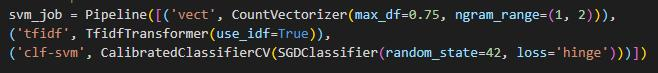
\includegraphics[width=1\textwidth]{chapter3/svm_pipline.jpg}  
    \caption{ตัวอย่างโค้ดไปป์ไลน์เทรนโมเดล}
    \label{Fig:svm_pipline}
  \end{figure}


\subsection{ระบบแนะนำ}

ระบบแนะนำ จะใช้เทคนิคการกรองโดยอิงจากเนื้อหาโดยเบสข้อมูลที่แตกต่างกันคือ ข้อมูลยูสเซอร์เบส และข้อมูลจ็อบเบส โดยการเลือกกลุ่มงานจะอ้างอิงจากระยะทางของยูสเซอร์และจ็อบด้วยระยะทางโคไซน์ (cosine distance) โดยการนำโมเดล SVM ที่เทรนจากข้อมูลที่แตกต่างกันมาเข้ามาใช้ในการทำนาย
\begin{algorithm}
  \DontPrintSemicolon
  \SetKwProg{Fn}{Function}{:}{}
  \Fn{Main(payload): Response(Record<string, any>[])}{
    read jobs from db\;
    read profiles from db\;
    load job-based pre-train model\;
    load profile-based pre-train model\;
    load accuracy weight by model

    return recommendation([job model, profile model], payload, jobs, acc, 20)
  }

  \SetKwProg{Fn}{Function}{:}{}
  \Fn{recommendation(models, payload, jobs, acc, n): Record<string, any>[]}{
    
    payload = clean payload text\;
    groups = predict `payload` in each `models'\;
    jobs = filter all jobs by groups(labels)\;
    acc = calculate accuracy in each group by weight 100\% \;
    jobs\_sim = calculate similarity between all job and payload then drop duplicate\;
    result = sort similarity job jobs\_sim \;
    return result[:n]\;
  }

  \caption{Job recommendation algorithm}
\end{algorithm}

\begin{figure}[!h]
  \centering
  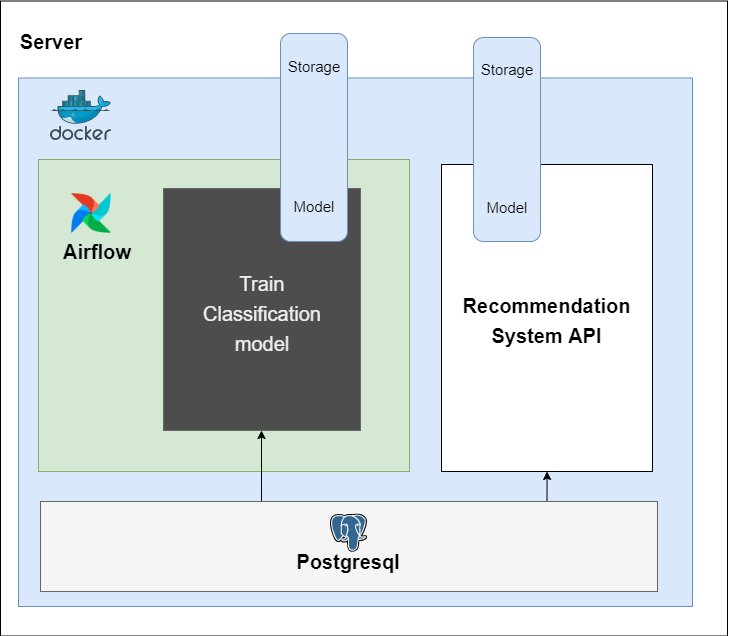
\includegraphics[width=0.7\textwidth]{structure_recomm.png}  
  \caption{รูปภาพโฟลว์การทำงานระบบแนะนำ}
  \label{Fig:strucutre_recomm}
\end{figure}


\pagebreak

\section{การพัฒนา API เพื่อให้บริการระบบแนะนำ}
ในการพัฒนา API เพื่อให้บริการระบบแนะนำนั้นผู้จัดทำได้เลือกเฟรมเวิร์คที่มีความคุ้นชินและเหมาะสมในการพัฒนามากที่สุดโดยเฟรมเวิร์คที่เลือกนั้นคือเฟรมเวิร์คของภาษา "python" ที่ชื่อว่า "flask" มาพัฒนาเป็น API โดยมีขั้นตอนดังนี้
\begin{enumerate}
  \itemsep0em 
  \item ออกแบบผังระบบ (Context Diagram)
  \item ผังการแยกฟังก์ชั่นงานย่อย (Decomposition Diagram)
  \item ออกแบบฐานข้อมูลเชิงคุณภาพ (Physical Design)
\end{enumerate}
\newpage

\subsection{ออกแบบผังระบบ (Context Diagram)}
  \begin{figure}[!h]
    \centering
    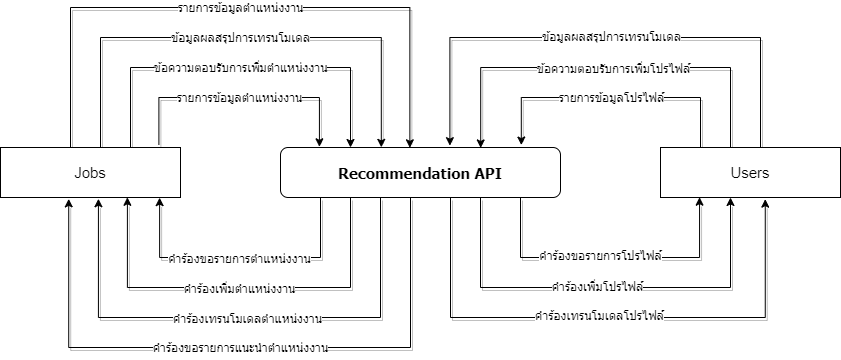
\includegraphics[width=1\textwidth]{chapter3/context-diagram.png}  
    \caption{context diagram}
    \label{Fig:context_diagram}
  \end{figure}

\subsection{ผังการแยกฟังก์ชั่นงานย่อย (Decomposition Diagram)}
  \begin{figure}[!h]
    \centering
    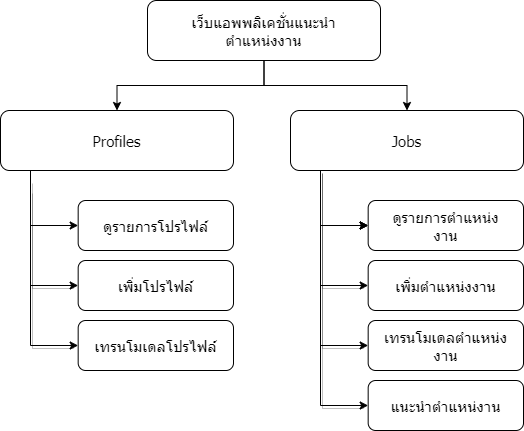
\includegraphics[width=0.8\textwidth]{chapter3/decomposiiton-diagram.png}  
    \caption{decomposiiton diagram}
    \label{Fig:decomposiiton_diagram}
  \end{figure}
  \newpage

\subsection{ออกแบบฐานข้อมูลเชิงคุณภาพ (Physical Design)}
\begin{figure}[!h]
  \centering
  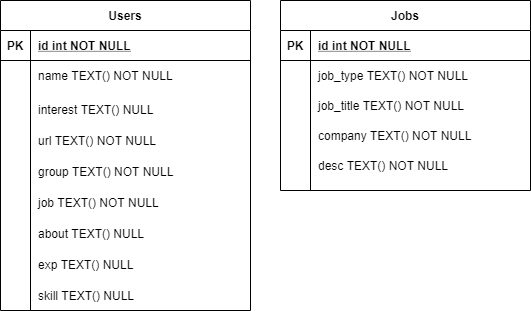
\includegraphics[width=0.8\textwidth]{chapter3/physical-diagram.png}  
  \caption{physical diagram}
  \label{Fig:physical_diagram}
\end{figure}



% \begin{figure}[!h]
%   \centering
%   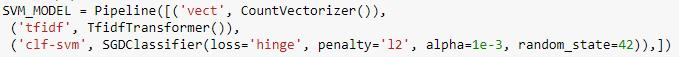
\includegraphics[width=0.95\textwidth]{model_pipeline.jpg}  
%   \caption{การสร้างขั้นตอนโมเดลด้วยไปป์ไลน์}
%   \label{Fig:data-prepare}
%   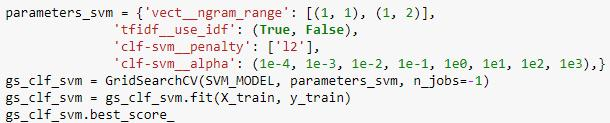
\includegraphics[width=0.95\textwidth]{model_optimize.jpg}  
%   \caption{การเลือกตัวแปรที่ดีที่สุดให้แก่โมเดล}
%   \label{Fig:data-prepare}
% \end{figure}




\chapter{ผลการทดลอง}

\section{การทำนายกลุ่มของโปรไฟล์}

\label{chapter:result}
ในส่วนนี้เรานำเสนอการทดลองเชิงประจักษ์ที่เน้นการประเมินคุณของการแนะนำงาน โดยการทดลองนี้เราได้มีข้อมูลโปลไฟล์ผู้เชี่ยวชาญจาก Linkedin จำนวน 417 ตัวอย่าง และตำแหน่งงานจาก Indeex จำนวน 4,748 ตำอย่าง, ทั้งโปรไฟล์และตำแหน่งงานเนื่องจากเฟิลด์ไอทีที่กว้างขวางโปรไฟล์จึงมีความแตกต่างกันบ้างเล็กน้อยในแต่ละกลุ่มโปรไฟล์ จากภาพด้านล่างแสดงการกระจายของฟิล์ดย่อยภายในของโปรไฟล์ 417 รายการซึ่งแสดงให้เห็นถึงจำนวนนักพัฒนาที่มีเป็นจำนวนมาก
\newline
\begin{figure}[!h]
  \centering
  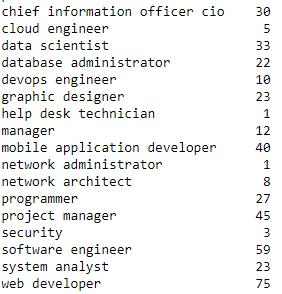
\includegraphics[width=0.5\textwidth]{profile_group.jpg}  
  \caption{การแยกกลุ่มของโปรไฟล์}
  \label{Fig:result-profile-group}
\end{figure}

ในการประเมินพวกเราได้ใช้ระบบแนะนำสร้างทำนายข้อมูลตำแหน่งงานสำหรับทดสอบ โดยใช้โมเดลที่ผ่านการเทรนมาแล้วได้โดยข้อมูลทดสอบนั้นเป็นข้อมูลรายละเอียดงานที่แบ่งมาจากส่วนเทรนจำนวน 33\% หรือ 1,567 ตัวอย่าง โดยจากรายงานการจำแนกประเภทเราจะเห็นว่าในกลุ่มตำแหน่งงานที่มีความคลุมเครือและใกล้เคียงกันเช่น 'web developer' และ 'software engineer' มีผลความแม่นยำที่น้อยเมื่อเทียบกับกลุ่มอื่น ๆ 

\begin{figure}[!h]
  \centering
  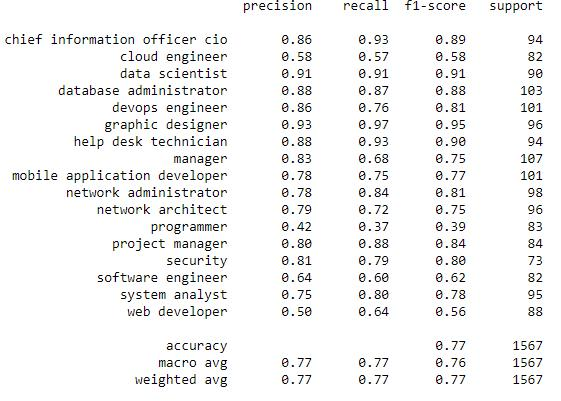
\includegraphics[width=0.95\textwidth]{classification_report.jpg}  
  \caption{รายงานการจำแนกประเภท}
  \label{Fig:result-classify-report}
\end{figure}

\newpage
ซึ่งจากการวิเคราะห์เราคาดว่าเกิดจากการใช้คำสำคัญ (keyword) ของโปรไฟล์ที่ดึงข้อมูลมาจาก linkedin โดยโปรไฟล์เหล่านี้มักใส่ทักษะวิชาชีพครอบคลุมในส่วนของการพัฒนาหรืออีกนัยคือ นักพัฒนาส่วนใหญ่เป็น full-stack ที่สามารถทำได้หลายตำแหน่งงาน แต่เนื่องจากตำแหน่งงานที่ทำในปัจจุบันของโปรไฟล์เหล่านั้นสามารถตั้งได้แค่ตำแหน่งเดียว ทำให้เกิดความคลาดเคลื่อนในการทำนาย
ทั้งนี้เมื่อเราทำการพล็อตการฟ confusion matrix เราจะเห็นถึงความผิดพลาดในการทำนายของตำแหน่ง 'software engineer' 'devops engineer' และ web developer เป็นจำนวนหนึ่งส่งผลให้ค่าความแม่นยำรวมเหลือแค่ 77\% ซึ่งทางเราถือว่าเกือบพอใช้ได้

\begin{figure}[!h]
  \centering
  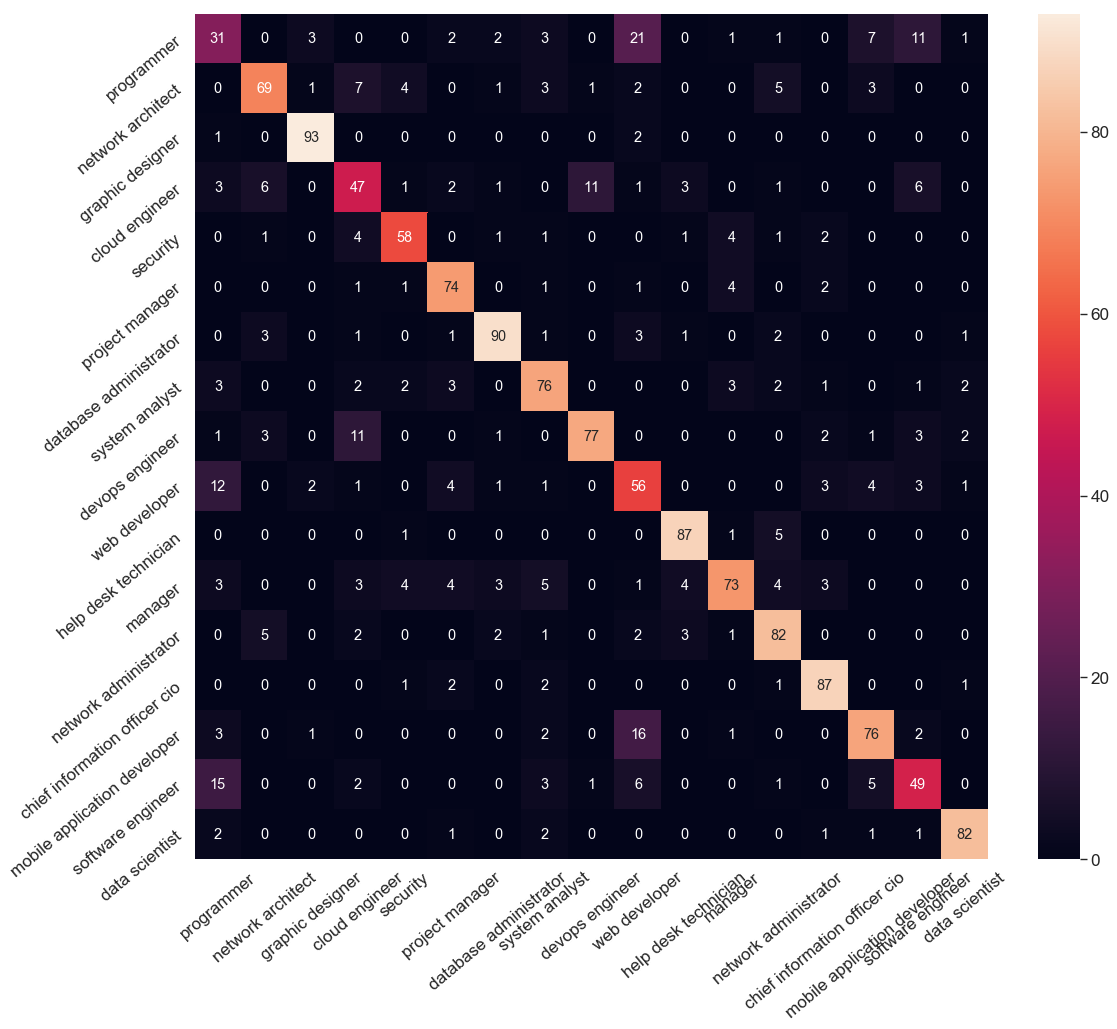
\includegraphics[width=1\textwidth]{confusion_matrix.png}  
  \caption{ตาราง confusion matrix}
  \label{Fig:result-classify-report}
\end{figure}

\newpage
\section{การจับคู่งานกับโปรไฟล์}
เราทำการแบ่งกลุ่มของโปรไฟล์ออกเป็นกลุ่มย่อย ๆ เนื่องจากในขั้นตอนการจับคู่งานกับโปรไฟล์โดยเทคนิคการหาระยะทางโคไซน์ (cosine distance) นั้นจำเป็นต้องใช้ทรัพย์ยากรเครื่องที่ประมวลผลเป็นจำนวนมาก การแบ่งกลุ่มออกเป็นกลุ่มย่อย ๆ จะช่วยแบ่งเบาภาระของการประมวลผลเพื่อหาตำแหน่งงานที่เหมาะสมกับโปรไฟล์ยูสเซอร์มากที่สุด

ผลลัพธ์การแนะนำตำแหน่งงานโดยการหาความสอดคล้องระหว่างโปรไฟล์ยูสเซอร์และงานในกลุ่ม เรายกตัวอย่างยูสเซอร์คนหนึ่งซึ่งเป็น senior software engineer ทำงานอยู่ agoda เพื่อเป็นตัวอย่างผลลัพธ์การแนะนำตำแหน่งงาน


\begin{figure}[!h]
  \centering
  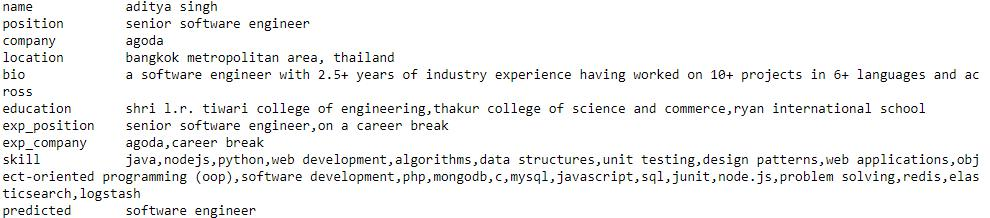
\includegraphics[width=1\textwidth]{user_example.jpg}  
  \caption{ตัวอย่างข้อมูลยูสเซอร์ในการแนะนำตำแหน่งงาน}
  \label{Fig:result-classify-report}
\end{figure}

\newpage

โดยเราทำการหา similarity distance ของตำแหน่งงานที่สอดคล้องกับโปรไฟล์นี้มากที่สุด 10 อันแรกจะได้ผลลัพธ์ตามนี้


\begin{figure}[!h]
  \centering
  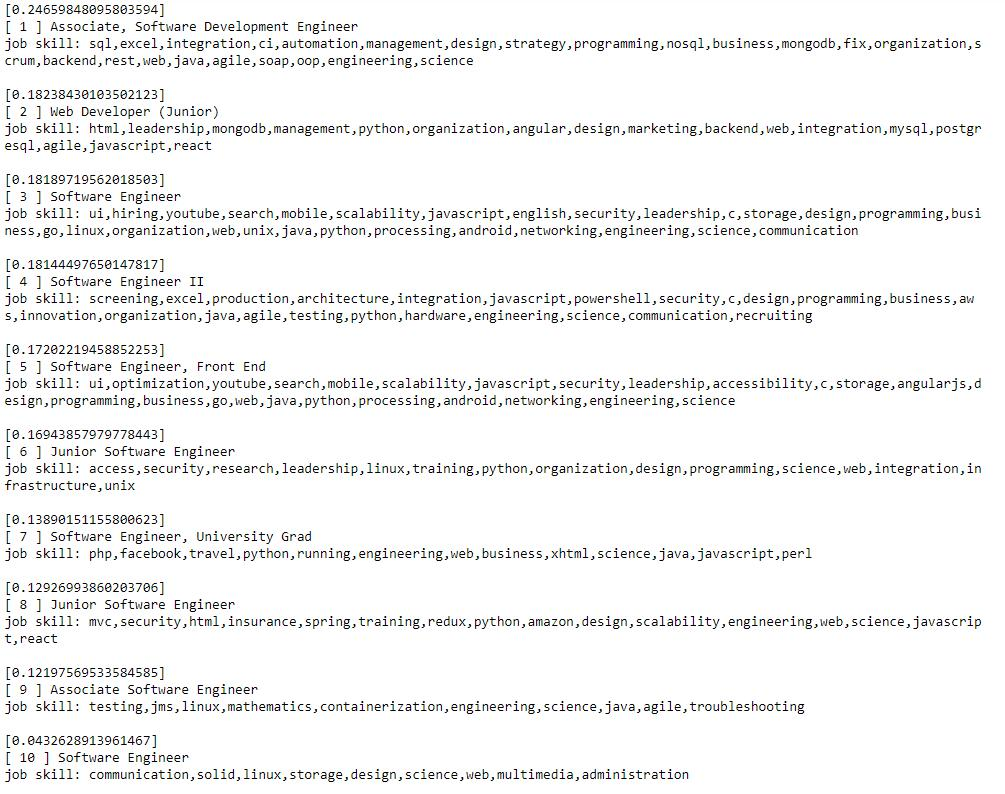
\includegraphics[width=1\textwidth]{recommend_result.jpg}  
  \caption{ผลการแนะนำตำแหน่งงานที่สอดคล้องกับยูสเซอร์มากที่สุด 10 อันแรก}
  \label{Fig:result-classify-report}
\end{figure}
\chapter{สรุปผล}
\label{chapter:conclusion}
ในการทดลองนี้ ได้เสนอกรอบการทำงานของระบบแนะนำตำแหน่งงานโดยใช้เทคนิคการกรองแบบเนื้อหา โดยใช้ข้อมูลที่แตกต่างกันสองแหล่งคือ จ็อบเบสหรือข้อมูลตำแหน่งงานและยูสเซอร์เบสหรือข้อมูลโปรไฟล์ผู้ใช้มาใช้ในการการเทรนโมเดลโดยใช้เทคนิค "Support vector machine" ซึ่งให้ผลลัพธ์ที่แม่นยำที่สุดเมื่อเทียบกับเทคนิคอื่น ๆ ผลลัพธ์ของโมเดลการแบ่งกลุ่มสายจะได้ความแม่นยำอยู่ที่ 86\% เมื่อใช้ข้อมูลจากตำแหน่งาน และ 49\% เมื่อใช้ข้อมูลยูสเซอร์ โดยความแม่นยำทั้งสองนี้จะถูกถ่วงน้ำหนักและสเกลด้วย 100 เพื่อใช้ในการแบ่งข้อมูลในขั้นตอนการแนะนำงานโดยผลลัพธ์ของตำแหน่งงานที่แนะนำมามีความแม่นยำอยู่ในระดับที่น่าพึงพอใจเป็นอย่างมาก ถึงแม้ว่าชื่อและประเภทงานอาจมีความคลาดเคลื่อน แต่เนื้อหาของงานค่อนข้างตรงกับการจับคู่กับโปรไฟล์ผู้ใช้

\section{ปัญหาที่เกิดขึ้น}
ปัญหาที่เกิดขึ้นจากการทดลอง ผู้จัดทำได้พบว่าข้อมูลที่สกัดมาจากเว็บไซต์ลิงค์อินนั้น โปรไฟล์ผู้ใช้มักเขียนคำอธิบานตนเองค่อนข้างไม่เกี่ยวข้องกับลักษณะงานที่ทำ อีกทั้งเว็บไซต์ลิงค์อินมีความยากในการสกัดข้อมูลเป็นอย่างมาก ทำให้ข้อมูลที่ได้นั้นมีจำนวนยังไม่เพียงพอต่อการใช้งานในความเห็นของผู้จัดทำ โดยปริมาณโปรไฟล์ที่สกัดมานั้นมีจำนวน 2,720 คน จากที่คาดหวังไว้ 6,000+ \par
ปัญหาต่อมาที่พบคือเนื่องจากตำแหน่งงานในแต่ละรายการนั้นมีความไม่เหมือนใครในด้านเนื้อหางานถึงแม้ว่าหัวข้อจะเหมือนกันก็ตาม รวมถึงตำแหน่งงานมีเวลาหมดอายุหรือปิดรับสมัคร ทำให้การแนะนำรายการเดิมนั้นเป็นไปไม่ได้ ทำให้การแนะนำด้วยเทคนิคการกรองแบบร่วมกัน ไม่สามารถใช้ได้ \par

\section{ทิศทางในอนาคต}
ทิศทางในอนาคตผู้จัดทำมุ่งเน้นไปที่เรื่องของข้อมูลที่ได้มามากกว่าตัวโมเดล โดยระบบสกัดข้อมูลที่ใช้อยู่ตอนนี้ยังไม่มีความไม่สเถียรและต้องมีการปรับปรุงอีกมากในการสกัดข้อมูลจากทั้งสองแหล่ง ผู้จัดทำจึงมีแผนในการพัฒนาโครงสร้างท่อข้อมูลให้เป็นระบบที่เป็นระบบอัตโนมัติ เพื่อให้ได้ข้อมูลที่ใหม่อยู่เสมอและความแม่นยำที่แม่นขึ้นในการแบ่งกลุ่มสายงาน


% \clearpage
\addcontentsline{toc}{chapter}{บรรณานุกรม}
\bibliographystyle{ieeetr}
\bibliography{reference}

\begin{thebibliography}{9}

  \bibitem{baptiste} 
  Baptiste Rocca: Introduction to recommender systems
  \\\texttt{https://towardsdatascience.com/introduction-to-recommender-systems-6c66cf15ada}

  \bibitem{tuple}
  Collaborative filtering ฟีเจอร์การแนะนำเพลงของ Spotify
  \\\texttt{https://tupleblog.github.io/spotify/}  

  \bibitem{robin} 
  Robin Burke : Hybrid Web Recommender Systems
  \textit{University of Colorado Boulder}

  \bibitem{Sharma} 
  Nikita Sharma: Recommender Systems with Python — Part I: Content-Based Filtering
  \\\texttt{https://heartbeat.fritz.ai/recommender-systems-with-python-part-i-content-based-filtering-5df4940bd831}

  \bibitem{princegrover} 
  Prince Grover: Various Implementations of Collaborative Filtering
  \\\texttt{https://towardsdatascience.com/various-implementations-of-collaborative-filtering100385c6dfe0}

  \bibitem{farshad} 
  Farshad Bakhshandegan Moghaddam : Cold Start Solutions For Recommendation Systems
  \textit{Institute for Automation and Applied Informatics}

  \bibitem{diego} 
  Diego Lopez Yse: Your Guide to Natural Language Processing (NLP)
  \\\texttt{https://towardsdatascience.com/your-guide-to-natural-language-processing-nlp-48ea2511f6e1}
  
  \bibitem{lukkiddd} 
  Lukkiddd: Word Embedding and Word2Vec
  \\\texttt{https://lukkiddd.com}

  \bibitem{cory} 
  Cory Maklin: TF IDF | TFIDF 
  \\\texttt{https://towardsdatascience.com/natural-language-processing-feature-engineering-using-tf-idf-e8b9d00e7e76}
  
  \bibitem{selva} 
  Selva Prabhakaran: Cosine Similarity – Understanding the math and how it works
  \\\texttt{https://www.machinelearningplus.com/nlp/cosine-similarity/}

  \bibitem{cory2} 
  Cory Maklin: Support Vector Machine Python Example
  \\\texttt{https://towardsdatascience.com/support-vector-machine-python-example-d67d9b63f1c8}

  \bibitem{choochart} 
  Choochart Haruechaiyasak: A Data Mining Framework for Building A Web-Page Recommendem System
  \textit{Information Research and Development Division. 2015}

  \bibitem{margaret} 
  Margaret Rouse: Web application
  \\\texttt{https://searchsoftwarequality.techtarget.com/definition/Web-application-Web-app}






  \bibitem{huizhiliang} 
  Huizhi Liang: Real-time Collaborative Filtering Recommender Systems
  \textit{Department of Computing and Information Systems}
  The University of Melbourne. 2005.

  \bibitem{philip} 
  Philip Lenhart: Combining Content-based and Collaborative Filtering for Personalized Sports News Recommendations
  \textit{Department of Informatics. 2016}

  \bibitem{PyOhio} 
  PyOhio Lenhart: “Large-Scale Recommendation System with Python and Spark
  \\\texttt{https://www.youtube.com/watch?v=oAByzl71Ak4}

  \bibitem{cory} 
  Cory Maklin: Support Vector Machine Python Example
  \\\texttt{https://towardsdatascience.com/support-vector-machine-python-example-d67d9b63f1c8}

  \bibitem{min} 
  Sung-Hwan Min: Recommender Systems Using Support Vector Machines 
  \textit{Graduate School of Management, Korea Advanced Institute of Science and Technology}
  207-43 Cheongrangri-dong, Dongdaemun-gu, Seoul 130-722, Korea shmin@kgsm.kaist.ac.kr 

  
  \bibitem{chhavi} 
  Chhavi Saluja: Collaborative Filtering based Recommendation Systems exemplified
  \\\texttt{https://towardsdatascience.com/collaborative-filtering-based-recommendation-systems-exemplified-ecbffe1c20b1}

  \bibitem{erion} 
  Erion Çano Min: Hybrid Recommender Systems: A Systematic Literature Review
  \textit{Charles University in Prague Prague, CZ, Czechia}

  \bibitem{adam} 
  Adam Lineberry: Hybrid Content-Collaborative Movie Recommender Using Deep Learning
  \\\texttt{https://towardsdatascience.com/creating-a-hybrid-content-collaborative-movie-recommender-using-deep-learning-cc8b431618af}

 
  \bibitem{qing} 
  Qing Li : An Approach for Combining Content-based and Collaborative Filters 
  \textit{Dept. of Computer Sciences Kumoh National Institute of Technology}
  Kumi, kyungpook, 730-701,South Korea liqing@se.Kumoh.ac.kr 

  \bibitem{jorge} 
  Jorge Valverde-Rebaza: Job Recommendation based on Job Seeker Skills: An Empirical Study
  \textit{Ricardo Puma's}

  \bibitem{airflow}
  Apache Airflow: Apache Airflow. Archived from the original on August 12, 2019. Retrieved September 30, 2019.
  \\\texttt{https://airflow.apache.org/docs/stable/project.html}

  \bibitem{docker}
  ทำความรู้จัก Docker และการใช้งานบน CentOS 7
  \\\texttt{https://www.hostpacific.com/using-docker-on-centos7/}

  \bibitem{comptia}
  CompTIA Certification Roadmap
  \\\texttt{http://certification.comptia.org/why-certify/roadmap}


  \end{thebibliography}

  

\newpage


% \startappendix
% % !TEX TS-program = xelatex
% !TEX encoding = UTF-8

\chapter{เรื่องที่หนึ่ง}

\end{document}